\documentclass[11pt,a4paper]{article}

% ---------- packages ----------
\usepackage[margin=2.5cm]{geometry}
\usepackage{setspace}
\usepackage{lineno}
\usepackage{graphicx}
\usepackage{booktabs}
\usepackage{array}
\usepackage{longtable}
\usepackage{pdflscape}
\usepackage[super,comma,sort&compress]{natbib}
\usepackage{caption}
\usepackage{amsmath}
\usepackage{textcomp}
\usepackage{microtype}
\usepackage{titlesec}
\usepackage[colorlinks=true,linkcolor=blue,citecolor=blue,urlcolor=blue,breaklinks]{hyperref}

\graphicspath{{../results/pub_figs/main/}{../results/pub_figs/supp/}{../results/pub_figs/}}
\bibliographystyle{unsrtnat}
\setlength{\bibsep}{1pt plus 0.3ex}

% journal-style headings and captions
\setcounter{secnumdepth}{0}
\titleformat{\section}{\large\bfseries}{}{0pt}{}
\titleformat{\subsection}{\normalsize\bfseries}{}{0pt}{}
\titlespacing*{\section}{0pt}{14pt}{6pt}
\titlespacing*{\subsection}{0pt}{10pt}{3pt}
\DeclareCaptionLabelSeparator{pipe}{ $\vert$ }
\captionsetup{labelfont=bf,labelsep=pipe,font=small,justification=justified,singlelinecheck=false}
\captionsetup[figure]{name=Fig.}



\begin{document}
\begin{flushleft}
{\LARGE\bfseries\linespread{1.1}\selectfont A cross-cohort single-cell reference atlas of H3K27-altered diffuse midline glioma\par}
\vspace{14pt}
{\large Md. Jubayer Hossain\textsuperscript{1,2,*} and Iqbal Mahmud\textsuperscript{3,*}\par}
\vspace{8pt}
{\small
\textsuperscript{1}Center for Health Innovation, Research, Action, and Learning -- Bangladesh\\
\textsuperscript{2}DeepBio\\
\textsuperscript{3}Department of Computational Biology and Bioinformatics, Lamar University\par}
\vspace{8pt}
{\small \textsuperscript{*}Joint correspondence:\\
Md. Jubayer Hossain, \href{mailto:contact.jubayerhossain@gmail.com}{contact.jubayerhossain@gmail.com}, ORCID: \href{https://orcid.org/0000-0001-9323-4997}{0000-0001-9323-4997}\\
Iqbal Mahmud, \href{mailto:imahmud1@lamar.edu}{imahmud1@lamar.edu}, ORCID: \href{https://orcid.org/0000-0001-7729-8122}{0000-0001-7729-8122}\par}
\end{flushleft}
\vspace{6pt}

% ================= ABSTRACT =================
\section{Abstract}
Diffuse midline glioma, H3 K27-altered (DMG), is a lethal brain tumour, mostly of children, whose single-cell data are
spread across small cohorts that differ in assay, anatomical site and clinical context. We integrated six public human
DMG datasets into a reference of 311,618 cells and nuclei from 57 samples and 52 patients. Copy-number-based malignant
calls agreed with the original annotations in a median 0.898 of cells per sample, and lineage labels transferred to
held-out patients with 0.975 accuracy. Under a replication rule specified before analysis, 2 of 15 malignant expression
metaprograms, cycling and hypoxia, recurred across three studies and in both cells and nuclei. Lineage-like programmes
were detected only in nuclei, and adding 22 whole-cell Smart-seq2 samples did not change this: lineage programme gene
content differed between platforms and cohorts. A ciliated programme carried the tumour's copy-number profile and is
therefore a tumour state. In 21 spatial transcriptomics sections from 12 patients, a pre-specified association between
mesenchymal-like tumour cells and myeloid cells was weak and an oligodendroglial association was absent. Refitting the reference without each study showed that malignant
and myeloid labels transfer to unseen studies, whereas rare normal lineages are frequently misclassified as malignant
(balanced accuracy 0.40--0.99 per held-out study), and that cycling is the only metaprogram recovered in every
scenario. The atlas defines which DMG cell states are reproducible across cohorts and provides openly available data,
reference models and code for mapping new samples.

\medskip
\noindent\textbf{Keywords:} diffuse midline glioma; H3 K27 alteration; single-cell RNA sequencing; single-nucleus RNA
sequencing; spatial transcriptomics; data integration; reference atlas

\newpage
\onehalfspacing
\linenumbers

% ================= INTRODUCTION =================
\section{Introduction}

Diffuse midline glioma, H3 K27-altered, is a World Health Organization (WHO) grade 4 tumour of the pons, thalamus and
spinal cord. Median survival is under one year, and no systemic therapy has improved it
\citep{louis2021who,mackay2017integrated,hoffman2018clinical}. Most tumours carry a lysine-to-methionine substitution at
position 27 of histone H3 (H3K27M) \citep{schwartzentruber2012driver,wu2012somatic}, which inhibits Polycomb repressive
complex 2 (PRC2) and causes global loss of H3K27 trimethylation with focal retention and widespread H3K27 acetylation
\citep{lewis2013inhibition,bender2013reduced,harutyunyan2019hkm,krug2019pervasive}. Transcriptional dependencies
\citep{nagaraja2017transcriptional}, electrical integration into neural circuits \citep{venkatesh2019electrical} and
subclonal functional diversity \citep{vinci2018functional} have been described, and cellular
immunotherapy has shown activity \citep{majzner2022gdcar}. The imipridone dordaviprone (ONC201) produced responses in
recurrent H3K27M-mutant DMG \citep{arrillagaromany2024onc} and received accelerated approval from the US Food and Drug
Administration in 2025 as the first systemic therapy for this tumour, but durable remission remains rare.

Single-cell RNA sequencing showed that DMG is dominated by oligodendrocyte-precursor-like (OPC-like) cells, with smaller
astrocyte-like (AC-like) and oligodendrocyte-like (OC-like) fractions \citep{filbin2018developmental}, a model later
refined by developmental anchoring \citep{jessa2022km,jessa2019stalled} and age-stratified analysis
\citep{liu2022landscape}. This hierarchy resembles that of adult glioblastoma \citep{patel2014singlecell,neftel2019integrative}.
The tumour microenvironment is non-inflammatory and dominated by microglia \citep{lin2018noninflammatory,ross2024microglia},
candidate immune checkpoints have been proposed \citep{collot2026igsfvista}, and spatial studies have begun to locate
tumour states in tissue \citep{ren2023spatial,huchede2024bmp}.

Three problems limit this literature. First, individual cohorts are small, so patient-level inference is rarely
possible. Second, deposits differ in ways that are confounded with biology: pontine tumours are often sampled at autopsy
and profiled as frozen nuclei \citep{okada2026singlenucleus}, whereas thalamic tumours are more often resected and
profiled as whole cells \citep{desisto2024tumor}. Third, tumour cell states are usually defined within a single study,
so it is unclear which reflect the disease and which reflect the protocol \citep{gavish2023hallmarks}. Integrated
reference atlases have addressed similar problems in other tissues and in adult glioblastoma
\citep{sikkema2023integrated,ruizmoreno2025gbmap}, but, to our knowledge, no cross-cohort reference has been
published for DMG.

Here we built such a reference and used it to test which findings hold across cohorts. We integrated six public
datasets with variational autoencoders \citep{lopez2018deep,xu2021probabilistic}, benchmarked the integration
\citep{luecken2021benchmarking} and projected five further cohorts onto it \citep{lotfollahi2021mapping}. We make four
contributions: (i) a harmonised 52-patient reference with calibrated malignant calls and reusable models; (ii) a
replication test of malignant expression programmes against a rule specified before analysis; (iii) patient-level
spatial tests of two pre-specified co-localisation hypotheses; and (iv) a leave-one-study-out evaluation that measures
what the reference can and cannot be trusted to do on new data.

% ================= RESULTS =================
\section{Results}

\subsection{An integrated reference of 52 patients}

We selected six public studies as the reference and reserved five further cohorts for projection only (Supplementary
Table~\ref{tab:deposits}). Of 420,381 cells in eligible samples, 356,406 (84.8\%) passed per-assay quality control. After
restriction to samples with unique molecular identifier (UMI) counts, the reference comprised \textbf{311,618 cells and
nuclei from 57 samples and 52 patients}, measured over 18,882 genes shared by all studies (Table~\ref{tab:cohort},
Fig.~\ref{fig:atlas}a). The post-mortem series of Okada et al.\ contributed half of the cells (156,936 nuclei from 22
patients) \citep{okada2026singlenucleus}, followed by the single-cell and multiome series of Jessa et al.\ (129,364 cells
from 23 patients) \citep{jessa2022km} and the cohorts of Collot et al.\ \citep{collot2026igsfvista}, Zang et al.\
\citep{zang2024singlecell} and DeSisto et al.\ \citep{desisto2024tumor}. Nuclei made up 88.4\% of the reference; 42 samples
were pontine and 15 thalamic. The H3 variant was reported for 32 of 57 samples (8 H3.1, 1 H3.2 and 23 H3.3).

We integrated the data with single-cell variational inference (scVI) \citep{lopez2018deep}, using sample as the batch
variable and study, assay and mitochondrial fraction as covariates, and benchmarked three random seeds against Harmony
\citep{korsunsky2019fast} and uncorrected principal components with single-cell integration benchmarking (scIB) metrics
\citep{luecken2021benchmarking}. A pre-specified score (0.4 $\times$ batch correction + 0.6 $\times$ biological
conservation, min--max scaled across candidates) selected seed 1, which scored 0.739 (batch 0.537, biology 0.874),
compared with 0.581 for Harmony and 0.126 for principal components (Fig.~\ref{fig:atlas}e, Supplementary
Fig.~\ref{sfig:2}). Lineage compartments separated clearly and studies intermixed within them
(Fig.~\ref{fig:atlas}b--d). Mixing across assays remained incomplete: the integration local inverse Simpson's index (iLISI)
for assay was 0.029 for the selected model and 0.134 for Harmony.

\begin{figure}[htbp]
\centering
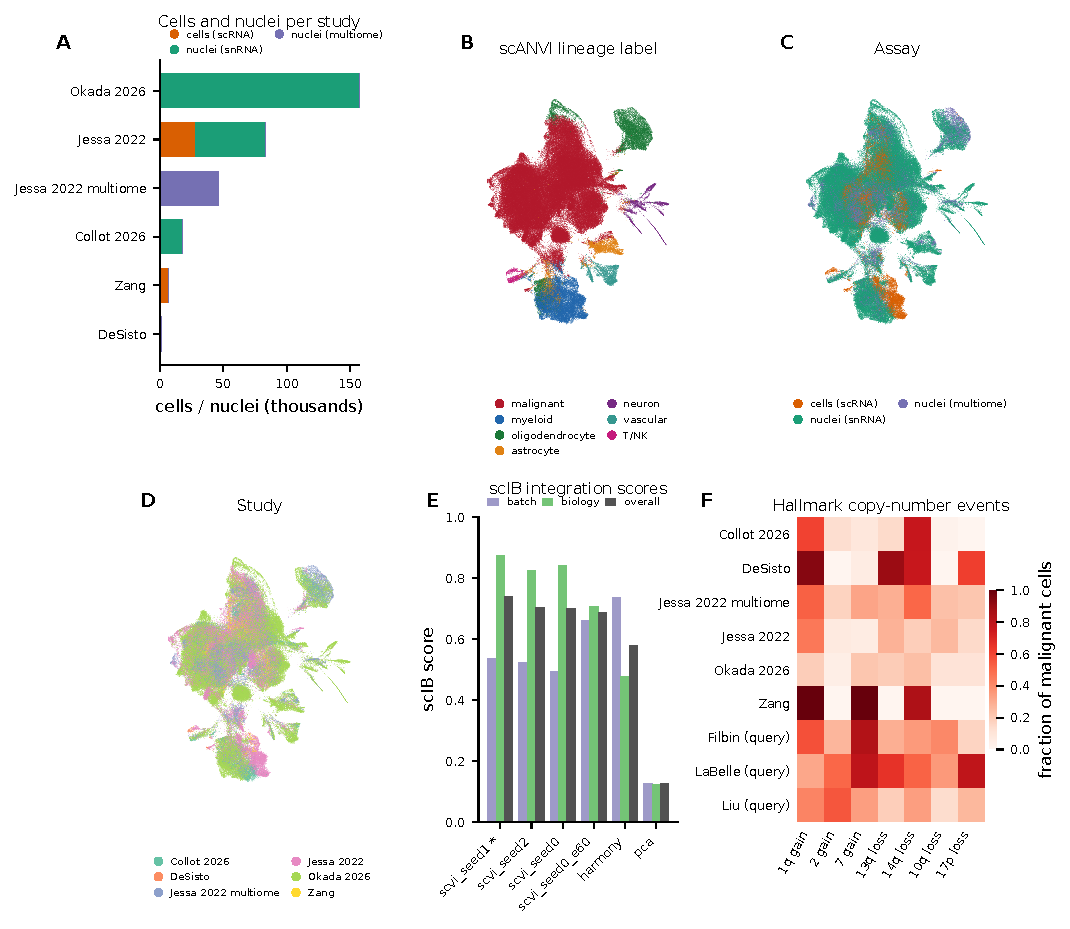
\includegraphics[width=\textwidth]{fig1_atlas.pdf}
\caption{\textbf{An integrated reference of H3 K27-altered diffuse midline glioma.} \textbf{a}, Cells and nuclei per
study, coloured by assay. \textbf{b--d}, UMAP of the scANVI latent space (311,618 cells, 57 samples, 52 patients)
coloured by lineage (b), assay (c) and study (d). \textbf{e}, scIB metrics for three scVI seeds, a 60-epoch scVI
sensitivity run, Harmony and uncorrected principal components; the asterisk marks the model selected by the
pre-specified score. \textbf{f}, Fraction of copy-number-malignant cells carrying each recurrent arm-level event, by
study, including the three projection-only tumour cohorts.}
\label{fig:atlas}
\end{figure}

\begin{table}[htbp]
\centering\footnotesize
\caption{\textbf{Reference cohort.} Samples, patients and cells per contributing study after quality control, with
assay, anatomical site and reported H3 variant (sample counts), and the fraction of cells called malignant by the
consensus rule. Counts are cells for whole-cell and nuclei for single-nucleus and multiome assays.}
\label{tab:cohort}
\resizebox{\textwidth}{!}{%
\begin{tabular}{lrrrlllr}
\toprule
Study & Samples & Patients & Cells & Assay (cells) & Site (samples) & H3 variant (samples) & Malignant \\
\midrule
Okada 2026 & 22 & 22 & 156,936 & snRNA:156936 & thalamus:6;pons:16 & unknown:22 & 0.516 \\
Jessa 2022 (sc/snRNA) & 17 & 17 & 83,076 & snRNA:54545;scRNA:28531 & pons:13;thalamus:4 & H3.1:6;H3.2:1;H3.3:10 & 0.566 \\
Jessa 2022 (multiome) & 10 & 10 & 46,288 & multiome\_RNA:46288 & pons:9;thalamus:1 & H3.1:2;H3.3:8 & 0.595 \\
Collot 2026 & 5 & 4 & 17,562 & snRNA:17562 & pons:3;thalamus:2 & H3.3:5 & 0.570 \\
Zang 2024 & 1 & 1 & 6,546 & scRNA:6546 & pons:1 & unknown:1 & 0.710 \\
DeSisto 2024 & 2 & 2 & 1,210 & scRNA:1210 & thalamus:2 & unknown:2 & 0.631 \\
\midrule
Total & 57 & 56 & 311,618 & \multicolumn{4}{l}{18,882 genes shared by all studies} \\
\bottomrule
\end{tabular}}
\end{table}


\subsection{Malignant calls agree with published labels}

Malignant status was assigned by combining lineage-marker scores with an expression-based copy-number profile computed
against normal cells of the same sample \citep{patel2014singlecell} (Methods). Across
\textbf{324,676 author-annotated cells in 97 samples}, the copy-number call agreed with the authors' labels in a median
\textbf{0.898} of cells per sample (interquartile range (IQR) 0.793--0.978; pooled agreement 0.884, precision 0.934,
recall 0.909; Table~\ref{tab:cnv}). Agreement in the 22 samples used to tune thresholds (0.882) was similar to that in
the 75 remaining samples (0.885). Calls supported by a recurrent arm-level event were more precise than calls based on
the aggregate score alone (0.952 versus 0.862), so event support is released as a confidence field.

Gain of chromosome 1q was the most frequent event, followed by loss of 14q and 13q (Fig.~\ref{fig:atlas}f). We excluded
4q12 from the event set because, at 100-gene resolution, it measures OPC-lineage expression rather than copy number.
Within the reference, the consensus of marker and copy-number evidence classified 170,940 cells as malignant (54.9\%),
50,754 as normal (16.3\%) and 89,924 as ambiguous (28.9\%). A permissive variant that accepts event-supported
copy-number calls classified a further 28,252 cells as malignant and is released as a sensitivity label.

\begin{table}[htbp]
\centering\footnotesize
\caption{\textbf{Agreement of malignant calls with published annotations.} Tier-2 comparison of the copy-number call
against each study's own annotation, for every annotated cell. Pooled values weight cells equally; the sample median
(with interquartile range) and unweighted sample mean weight samples equally.}
\label{tab:cnv}
\resizebox{\textwidth}{!}{%
\begin{tabular}{lrrrrrlr}
\toprule
Study & Cells & Samples & Agreement & Precision & Recall & Sample median (IQR) & Sample mean \\
\midrule
Jessa 2022 (sc/snRNA) & 84,194 & 17 & 0.915 & 0.982 & 0.914 & 0.898 (0.835--0.964) & 0.846 \\
Jessa 2022 (multiome) & 46,618 & 10 & 0.935 & 0.948 & 0.967 & 0.948 (0.897--0.988) & 0.930 \\
Collot 2026 & 17,750 & 5 & 0.907 & 0.896 & 0.975 & 0.960 (0.919--0.964) & 0.929 \\
Okada 2026 & 161,043 & 22 & 0.850 & 0.906 & 0.890 & 0.868 (0.763--0.895) & 0.800 \\
Liu 2022 (query) & 8,705 & 42 & 0.799 & 0.975 & 0.782 & 0.945 (0.770--0.990) & 0.813 \\
LaBelle (query) & 6,366 & 1 & 1.000 & nan & nan & 1.000 (1.000--1.000) & 1.000 \\
\textbf{\textbf{All}} & \textbf{324,676} & \textbf{97} & \textbf{0.884} & \textbf{0.934} & \textbf{0.909} & \textbf{0.898 (0.793--0.978)} & \textbf{0.836} \\
\bottomrule
\end{tabular}}
\end{table}


\subsection{Labels transfer to new patients and external cohorts}

A semi-supervised classifier (scANVI) \citep{xu2021probabilistic}, evaluated on five patients withheld from classifier
training, reached \textbf{0.975 accuracy} and 0.917 balanced accuracy on 23,827 cells. Recall ranged from 0.999 for
malignant cells to 0.803 for astrocytes (Supplementary Fig.~\ref{sfig:2}). Because the underlying scVI encoder had seen
these patients, this test measures generalisation to new patients from known studies; generalisation to new studies is
tested below.

We next projected five cohorts excluded from training through the frozen encoder without fine-tuning
(Fig.~\ref{fig:mapping}). Most cells of the two DMG cohorts deposited as transcripts per million (TPM) were classified as
malignant (median 90.3\% per sample for Filbin et al.\ \citep{filbin2018developmental} and 83.6\% for the 42 samples from 41
patients of Liu et al.\ \citep{liu2022landscape}), and 95.1\% of the cells that Liu et al.\ annotated as malignant were
classified as malignant. In the immune-focused cohort of LaBelle et al.\ \citep{labelle2025dissecting}, the median per-sample malignant fraction
was 49.9\% and the pooled fraction 11.1\%. Adult pons nuclei \citep{siletti2023transcriptomic} were classified as
malignant in a median of 1.2\% of cells, whereas fetal hindbrain cells \citep{braun2023comprehensive} were classified as
malignant in a median of 91.3\%. The reference contains no normal progenitor class, so fetal radial glia, glioblasts and
neuroblasts were assigned to the nearest available class. Their median distance to the 15 nearest reference cells was 2.60,
compared with 1.57 among reference cells, but the TPM cohorts showed similarly high mapping uncertainty, so neighbour distance alone
does not identify this failure (Supplementary Fig.~\ref{sfig:3}).

\begin{figure}[htbp]
\centering
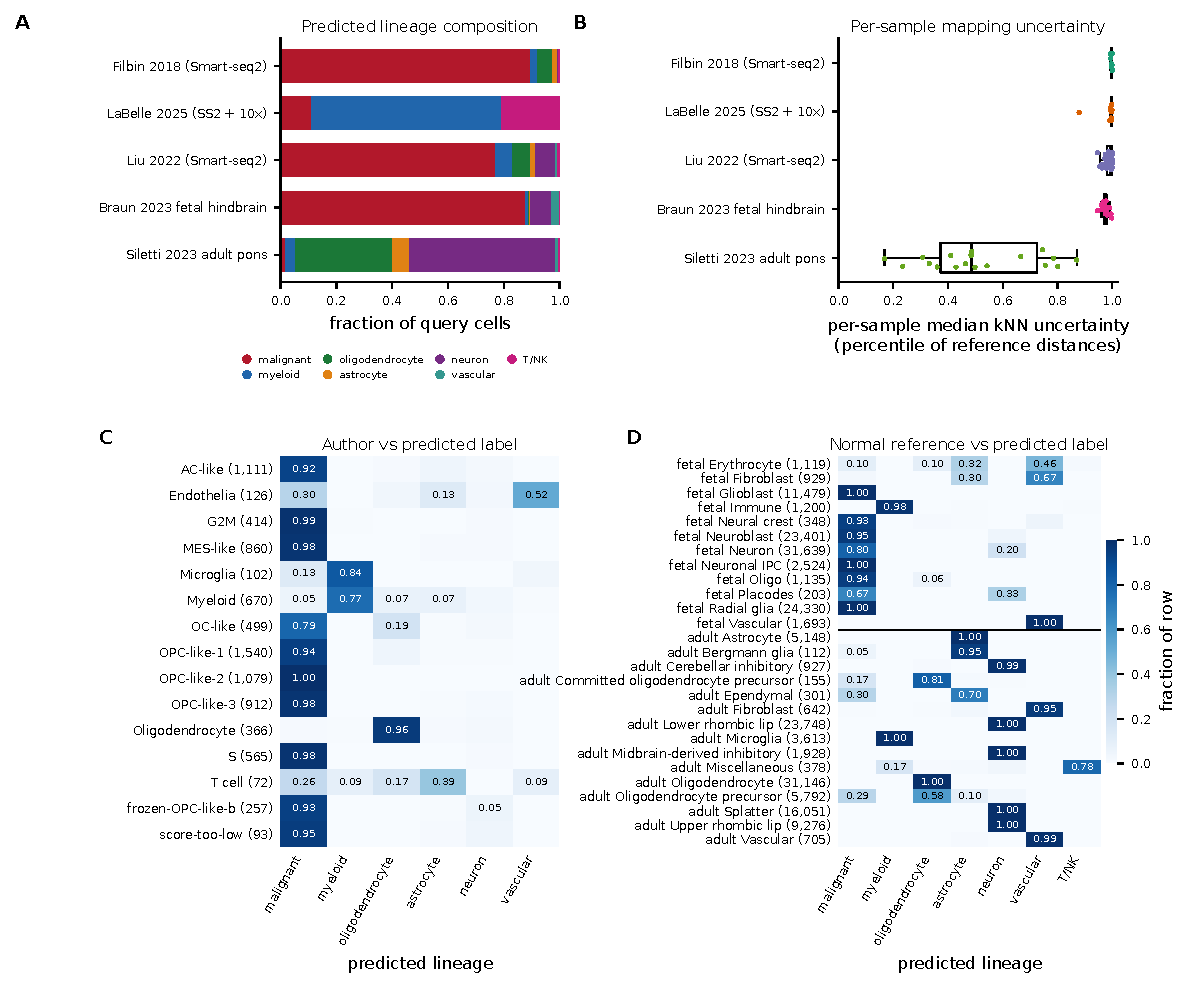
\includegraphics[width=\textwidth]{fig2_mapping.pdf}
\caption{\textbf{Zero-shot projection of five external cohorts.} \textbf{a}, Predicted lineage composition of each query
cohort. \textbf{b}, Per-sample median neighbour-based uncertainty, expressed as a percentile of the reference's own
15-nearest-neighbour distances. \textbf{c}, Author-annotated state against predicted lineage for Liu et al.\
(row-normalised). \textbf{d}, Fetal (Braun et al.) and adult (Siletti et al.) reference classes against predicted
lineage.}
\label{fig:mapping}
\end{figure}

\subsection{Two of 15 metaprograms replicate}

Consensus non-negative matrix factorisation (cNMF) \citep{kotliar2019identifying} of 167,012 malignant cells from 50
samples yielded per-sample expression programmes, which we clustered into 15 metaprograms, that is, programmes recurring
across samples (Table~\ref{tab:mp}, Fig.~\ref{fig:mp}a, Supplementary Fig.~\ref{sfig:4}). Twelve had a lineage-like
identity and three were technical (ribosomal, mitochondrial and dissociation stress). Under the pre-specified rule, a
metaprogram replicates if it recurs in at least three studies and in both cells and nuclei. \textbf{Two metaprograms
replicated}: cycling (MP1, 34 samples) and hypoxia (MP4, 15 samples). Both also replicated under a stricter rule requiring at least two samples per assay
class. This count was stable across dendrogram cuts from
0.84 to 0.90 (Supplementary Fig.~\ref{sfig:4}c).

Every lineage-like metaprogram was detected only in nuclei, and the only programme restricted to whole cells reflected
dissociation stress. Only six whole-cell samples from three publications contributed to programme discovery, so we
tested whether more whole-cell data would change this. We factorised the malignant cells of the Smart-seq2 cohorts of
Filbin et al.\ and Liu et al., in which the OPC-like, AC-like and OC-like states were first described (31 samples with at
least 100 malignant cells: 22 whole-cell and 9 nucleus samples), and re-clustered their programmes together with the 400
primary programmes using the unchanged rule. Cycling and hypoxia again replicated, now with 27 and 6 whole-cell samples,
but none of the primary lineage-like metaprograms acquired a whole-cell member. Instead, a whole-cell astrocyte-like
metaprogram emerged (\textit{AQP4}, \textit{SPARCL1}, \textit{CLU}, \textit{GFAP}, \textit{APOE}; 7 whole-cell samples
from three publications), which did not match the nucleus-derived AC-like metaprograms and did not replicate under the
stricter rule because it contained a single nucleus sample. Smart-seq2 nucleus programmes also rarely resembled the 10x
nucleus metaprograms (2 of 47 with Jaccard similarity of at least 0.15). The gene content of lineage-like programmes
therefore differs between platforms and cohorts, and not only between cells and nuclei. Masking 6,013 genes that differ between paired cells and nuclei yielded 12
metaprograms, 3 of which replicated: cycling, hypoxia and an OPC-like metaprogram derived mainly from MP3. The OPC-like
metaprogram included a single whole-cell sample and did not replicate under a stricter rule requiring at least two samples
per assay class, under which 2 metaprograms replicated. Random masks of the same size left a median of 2.5 metaprograms,
1 of which replicated; because random masks removed far more programme structure, this control does not isolate the
effect of assay-biased genes (Fig.~\ref{fig:mp}b, Supplementary Fig.~\ref{sfig:5}). The ciliated metaprogram (MP9; \textit{ADGB},
\textit{CFAP43}, \textit{DNAH9}) consists of motile-cilia genes that are also expressed by normal ependymal cells. Cells
scoring highly for MP9, however, carried the copy-number profile of the tumour: in all 33 samples with enough such cells,
their arm-level profile matched that of the other malignant cells of the sample (median tumour index 0.97, with 1 for the
other malignant cells and 0.03 for normal reference cells), and a median of 92\% lay above the 95th percentile of normal
reference cells. MP9 is therefore a ciliated tumour state rather than ependymal contamination.

\begin{figure}[htbp]
\centering
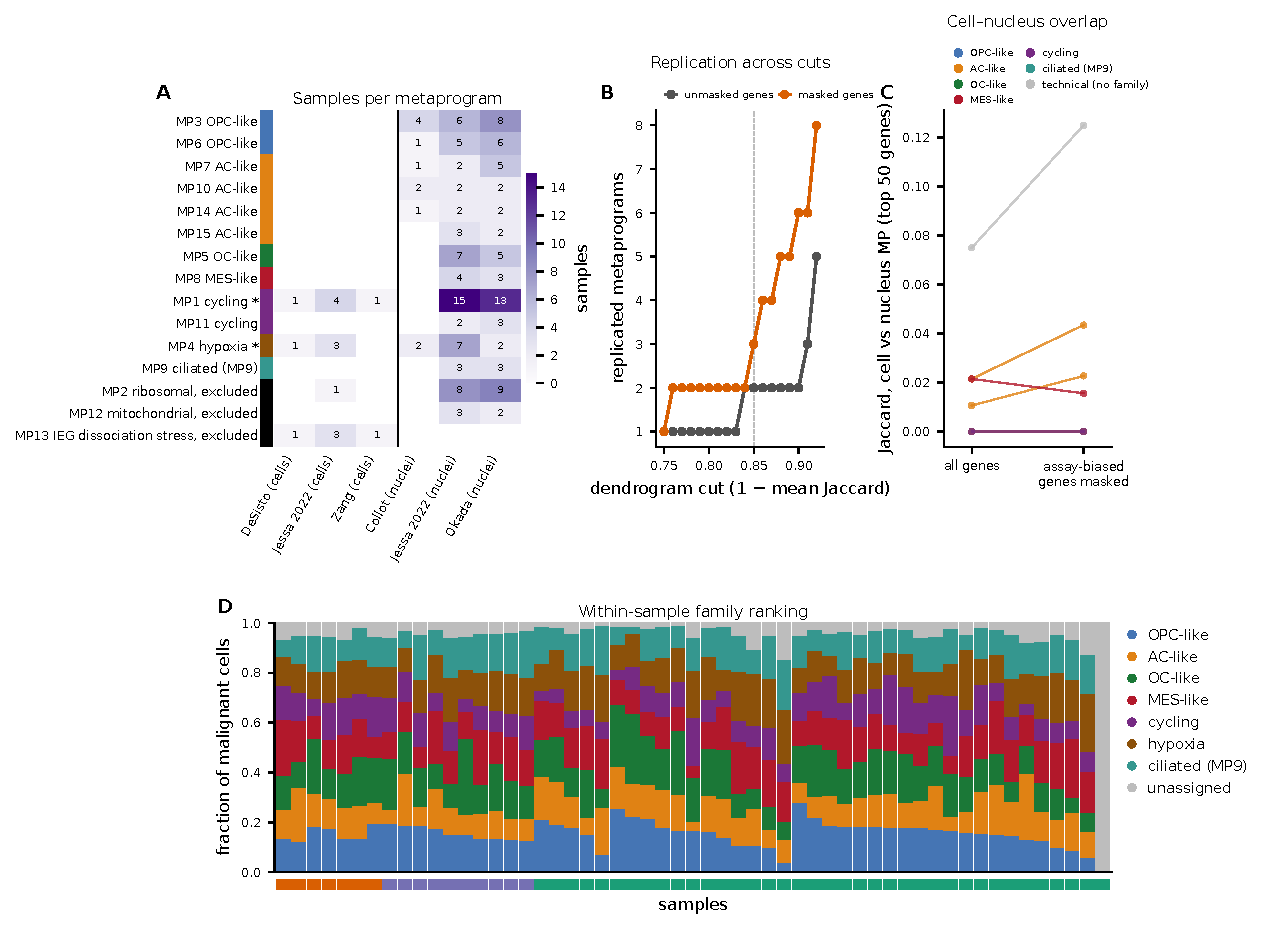
\includegraphics[width=\textwidth]{fig3_metaprograms.pdf}
\caption{\textbf{Metaprograms and their assay dependence.} \textbf{a}, Metaprogram occurrence by study and assay;
replicated metaprograms are marked and technical programmes are labelled. \textbf{b}, Replicated metaprograms across
dendrogram cuts, with and without masking the 6,013 assay-biased genes; the dashed line marks the primary cut.
\textbf{c}, Jaccard similarity of matched cell- and nucleus-derived metaprograms before and after masking. \textbf{d},
Per-sample distribution of malignant cells across metaprogram families. Families are assigned from scores standardised
within each sample, so this panel shows the relative ranking of programmes within samples, not absolute family
abundance.}
\label{fig:mp}
\end{figure}

\begin{table}[htbp]
\centering\footnotesize
\caption{\textbf{Consensus metaprograms.} Metaprograms at the primary dendrogram cut, their assigned lineage family or
technical class, the number of samples in which a contributing programme was found, whether they satisfy the
pre-specified replication rule (at least three studies and both assay classes), and their top genes.}
\label{tab:mp}
\resizebox{\textwidth}{!}{%
\begin{tabular}{llrll}
\toprule
Metaprogram & Family & Samples & Replicated & Top genes \\
\midrule
MP1 & cycling & 34 & yes & \textit{ASPM, TOP2A, CENPF, MKI67, KIF14, TPX2} \\
MP2 & \textit{ribosomal} & 18 & no & \textit{RPL32, RPS18, RPS8, RPS27, EEF1A1, RPL8} \\
MP3 & OPC-like & 18 & no & \textit{FGF12, DSCAM, TNR, CA10, DCC, CADM2} \\
MP4 & hypoxia & 15 & yes & \textit{SLC6A6, NDRG1, AKAP12, VEGFA, HILPDA, IGFBP5} \\
MP5 & OC-like & 12 & no & \textit{TNS3, BCAS1, OPCML, GPR17, PKP4, FGF12} \\
MP6 & OPC-like & 12 & no & \textit{LHFPL3, SEZ6L, LRRC4C, KCNIP4, MMP16, SEMA5A} \\
MP7 & AC-like & 8 & no & \textit{DAAM2, NKAIN3, MGAT4C, EEPD1, DCLK1, SLC4A4} \\
MP8 & MES-like & 7 & no & \textit{CD44, NAMPT, HRH1, SAMD4A, TGFB2, TPST1} \\
MP9 & ciliated (MP9) & 6 & no & \textit{ADGB, CFAP43, DNAH9, ZBBX, MAP3K19, CFAP299} \\
MP10 & AC-like & 6 & no & \textit{SLC4A4, EEPD1, FAT3, PTPRT, ADGRV1, SLC1A3} \\
MP11 & cycling & 5 & no & \textit{BRIP1, DTL, CENPP, CENPK, RFC3, MMS22L} \\
MP12 & \textit{mitochondrial} & 5 & no & \textit{MT-CO2, MT-ND4, MT-CO3, MT-ND3, MT-CYB, MT-ATP6} \\
MP13 & \textit{IEG / dissociation stress} & 5 & no & \textit{IER2, FOS, JUNB, EGR1, JUN, FOSB} \\
MP14 & AC-like & 5 & no & \textit{DCLK1, EEPD1, SORBS1, AQP4, DAAM2, RGMA} \\
MP15 & AC-like & 5 & no & \textit{EEPD1, CD44, SPARCL1, SORBS1, SLC4A4, TNC} \\
\bottomrule
\end{tabular}}
\end{table}


\subsection{Microenvironment and composition}

Subclustering resolved 21 microenvironment populations, including homeostatic microglia, three tumour-associated
macrophage states, CD4$^{+}$ and CD8$^{+}$ T cells, natural killer cells, five vascular populations and five
oligodendroglial states (Fig.~\ref{fig:tme}a, Supplementary Fig.~\ref{sfig:6}). This composition is consistent with a
myeloid-dominated, lymphocyte-poor microenvironment \citep{lin2018noninflammatory,ross2024microglia}. Several
populations were derived almost entirely from nuclei (Fig.~\ref{fig:tme}b).

Across samples, neurons were more abundant in H3.1 than in H3.3 tumours (change in logit proportion 2.60, $q = 0.004$;
site-adjusted $q = 0.017$; pons only $q = 0.050$). All H3.1 samples, however, were pontine nuclei from a single
publication, so this difference cannot be separated from study. Astrocytes (change in logit proportion 1.76,
$q = 0.038$) and myeloid cells (1.85, $q = 0.038$) were also more abundant in H3.1 tumours, but neither remained
significant after adjustment for site ($q = 0.167$). Among microenvironment subclusters, one mature-oligodendrocyte
subcluster was more abundant in H3.1 tumours ($q = 0.011$; site-adjusted $q = 0.009$), and several oligodendroglial and
vascular subclusters differed between the 6 adult and 46 paediatric patients ($q < 0.05$). All composition results are
provided in Supplementary Data~6. The largest compositional difference was technical: neurons were more abundant in nuclei than
in whole cells (change in logit proportion 3.40, $q < 10^{-9}$; Fig.~\ref{fig:tme}c).

\begin{figure}[htbp]
\centering
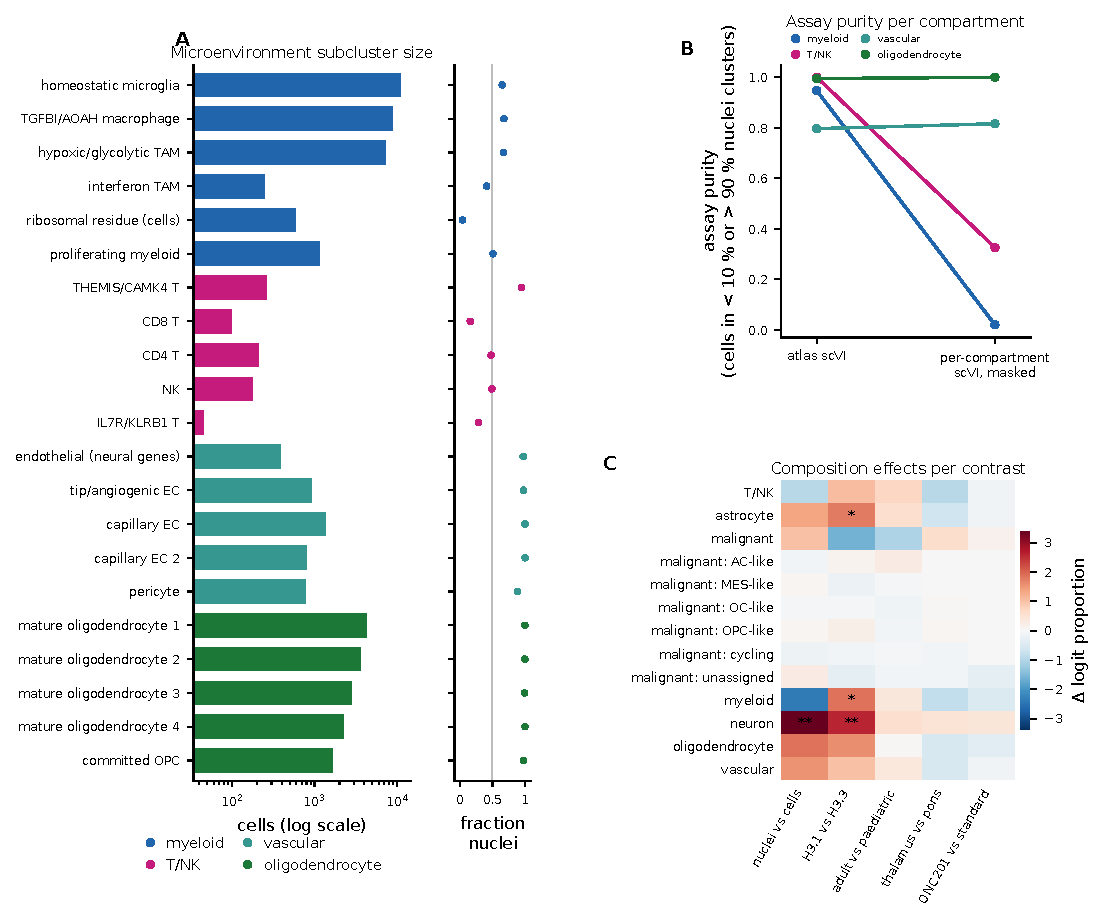
\includegraphics[width=\textwidth]{fig4_tme.pdf}
\caption{\textbf{Microenvironment populations and sample-level composition.} \textbf{a}, Microenvironment subclusters:
cell count (log scale) and fraction derived from nuclei. \textbf{b}, Assay purity of microenvironment clusters in the
atlas embedding and in a per-compartment model. \textbf{c}, Composition contrasts as change in logit proportion;
asterisks mark Benjamini--Hochberg significance \citep{benjamini1995controlling}.}
\label{fig:tme}
\end{figure}

\subsection{Spatial co-localisation of malignant states}

We deconvolved 27 Visium spatial transcriptomics sections from four cohorts with cell2location
\citep{kleshchevnikov2022celllocation}, using a 13-class reference, and tested co-localisation on spot proportions with
patients as the unit of inference (21 DMG sections from 12 patients; Table~\ref{tab:spatial}, Fig.~\ref{fig:spatial}).
AC-like tumour cells co-localised with normal astrocytes ($\rho = 0.393$, $q < 0.001$) and oligodendrocytes
($\rho = 0.308$, $q = 0.005$). Of the two pre-specified hypotheses, mesenchymal-like (MES-like) tumour cells co-localised
with myeloid cells ($\rho = 0.238$, 95\% confidence interval (CI) 0.071--0.392, $q = 0.034$), whereas OPC-like tumour
cells and oligodendrocytes were not associated ($\rho = 0.178$, 95\% CI $-0.028$ to 0.370, $q = 0.210$). These associations were
not consistent across sections: the correlation was positive in 13, 14 and 11 of 21 sections for the three pairs, the
mean per-section correlations (0.130, 0.171 and 0.079) were smaller than the pooled estimates, and heterogeneity between
patients was high for every pair ($I^2$ 0.952--0.997). Because DerSimonian--Laird intervals are too narrow with few
patients, we recomputed them with the Hartung--Knapp--Sidik--Jonkman method. Three pairs remained significant across the
42 pairs (ciliated--astrocyte, ciliated--neuron and AC-like--astrocyte; $q = 0.027$--$0.039$). The MES-like--myeloid
interval was 0.047--0.412 ($P = 0.020$), significant as one of two pre-specified hypotheses (Bonferroni-adjusted
$P = 0.039$) but not after correction across all 42 pairs ($q = 0.118$); these associations should therefore be regarded
as tentative (Supplementary Fig.~\ref{sfig:7}). Deconvolution can also create correlations between classes with similar
reference signatures: across the 42 pairs, the pooled correlation increased with the similarity of the two classes'
signatures (Spearman 0.53, $P < 0.001$). The MES-like and myeloid signatures (cosine similarity $-0.38$) and the AC-like and
astrocyte signatures ($-0.05$) were dissimilar, whereas the ciliated and astrocyte signatures were the most similar of all
pairs (0.17), so the ciliated--astrocyte association may partly reflect signature overlap. With
centred log-ratio-transformed proportions, the MES-like--myeloid ($\rho = 0.238$, $q = 0.012$) and AC-like--astrocyte
($\rho = 0.230$, $q = 0.001$) associations persisted, the AC-like--oligodendrocyte association weakened ($\rho = 0.129$,
$q = 0.048$), and the OPC-like--oligodendrocyte association was absent ($\rho = 0.007$, $q = 0.937$).

In ten sections from different levels of one brainstem autopsy (medulla, pons, midbrain and spinal cord)
\citep{kordowski2025spatial}, tumour fraction increased with the AC-like and OPC-like shares and
decreased with the normal glial, vascular and neuronal shares; with a single patient, this observation is descriptive.
Five DMG and five glioblastoma sections from one study \citep{ren2023spatial} differed in tumour fraction (0.528 versus
0.460) and cycling share (0.112 versus 0.214), but neither difference was significant after correction ($q = 0.667$).

\begin{figure}[htbp]
\centering
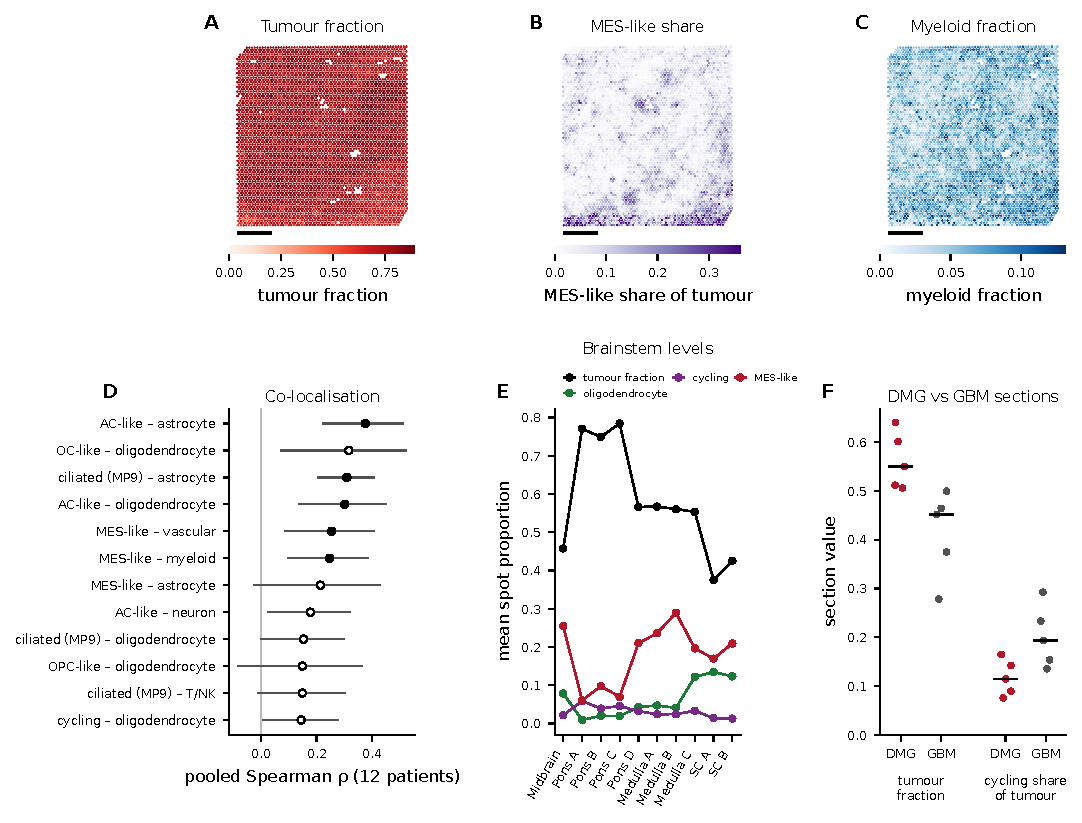
\includegraphics[width=\textwidth]{fig5_spatial.pdf}
\caption{\textbf{Spatial organisation of malignant states.} \textbf{a--c}, A representative section (scale bar, 1\,mm)
showing tumour fraction, the mesenchymal share of tumour and myeloid fraction. \textbf{d}, Pooled spot-level Spearman
correlations between malignant states and microenvironment lineages (12 patients, 21 sections); filled points are
significant after Benjamini--Hochberg correction across 42 pairs. \textbf{e}, Mean spot proportions in ten sections
from different brainstem levels of one autopsy. \textbf{f}, Tumour fraction and cycling share in five DMG and five glioblastoma sections from
one study.}
\label{fig:spatial}
\end{figure}

\begin{table}[htbp]
\centering\footnotesize
\caption{\textbf{Spatial co-localisation of malignant states with microenvironment lineages.} Spot-level Spearman
correlations of cell2location proportions, Fisher-$z$ averaged within patient and pooled by random effects over 12 DMG
patients and 21 sections, Benjamini--Hochberg corrected across 42 state-by-microenvironment pairs. The ten strongest
pairs are shown; $I^2$ quantifies between-patient heterogeneity.}
\label{tab:spatial}
\resizebox{\textwidth}{!}{%
\begin{tabular}{llrlrrr}
\toprule
Malignant state & Lineage & $\rho$ & 95\% CI & $q$ & Sections $>0$ & $I^2$ \\
\midrule
AC-like & astrocyte & 0.393 & 0.234 to 0.531 & 9.38e-05 & 13/21 & 0.993 \\
ciliated (MP9) & neuron & 0.230 & 0.131 to 0.324 & 9.38e-05 & 16/21 & 0.978 \\
ciliated (MP9) & astrocyte & 0.369 & 0.216 to 0.505 & 9.38e-05 & 13/21 & 0.992 \\
AC-like & oligodendrocyte & 0.308 & 0.138 to 0.459 & 0.00512 & 11/21 & 0.993 \\
MES-like & vascular & 0.253 & 0.078 to 0.412 & 0.0339 & 13/21 & 0.993 \\
MES-like & myeloid & 0.238 & 0.071 to 0.392 & 0.0339 & 14/21 & 0.992 \\
ciliated (MP9) & oligodendrocyte & 0.235 & 0.073 to 0.385 & 0.0339 & 13/21 & 0.992 \\
OC-like & vascular & -0.214 & -0.367 to -0.051 & 0.0511 & 6/21 & 0.993 \\
ciliated (MP9) & T/NK & 0.188 & 0.044 to 0.324 & 0.0511 & 14/21 & 0.990 \\
hypoxia & T/NK & 0.082 & 0.017 to 0.147 & 0.0589 & 12/21 & 0.952 \\
\bottomrule
\end{tabular}}
\end{table}


\subsection{Robustness to removing one study}

Two publications contributed 92\% of the cells, so we repeated the central analyses with each of the five publications
removed in turn; the two Jessa et al.\ series share four patients and were treated as one publication.

For label transfer, scVI and scANVI were retrained without the held-out publication, which was then mapped by
architectural surgery \citep{lotfollahi2021mapping} with its labels hidden. Accuracy, computed on cells with a malignant or normal consensus label, remained between 0.880 and 0.992,
but balanced accuracy ranged from 0.402 to 0.988 (0.506 when all folds were pooled by cell, compared with 0.917 for held-out
patients;
Fig.~\ref{fig:robust}a,b). Malignant (recall 0.86--1.00) and myeloid (recall 0.98--1.00) labels transferred to every
study, whereas astrocyte recall ranged from 0.00 to 0.56 and T and natural killer cells were mostly classified as myeloid.
Errors favoured the malignant class: when the post-mortem series was held out, 98\% of its neurons (3,838 of 3,898), 63\%
of its astrocytes and 51\% of its vascular cells were classified as malignant (Fig.~\ref{fig:robust}c). In this fold,
the errors were made with high confidence: accuracy among predictions with probability of at least 0.9 was 0.912.
Because this series contributes half of the reference, holding it out also halves the training data, so the drop in
performance reflects both study shift and reduced training size.

For metaprograms, we repeated the clustering without each publication, in 20 publication-balanced pools of at most five
samples per publication, and in 20 random pools of the same size. Cycling (MP1) was the only metaprogram recovered in every scenario and replicated in
all 20 balanced pools; three further metaprograms (ribosomal MP2, OC-like MP5 and OPC-like MP6) were recovered whenever a
single publication was removed but not in most smaller pools. Hypoxia (MP4) was lost when the Jessa et al.\ series was removed and replicated in
only 4 of 20 balanced pools. The MES-like and ciliated metaprograms, and four others, were recovered only when both large
series were present (Fig.~\ref{fig:robust}d).

For composition, we relabelled the ambiguous cells (28.9\% of the reference) in three ways: consensus labels only, ambiguous as a
separate category, and confident scANVI labels only. All four significant effects remained significant and retained
their sign under every labelling (Fig.~\ref{fig:robust}e).

Finally, we asked whether per-cell metaprogram-family assignments measure composition, by testing whether a sample's
fraction of a family was higher when the sample's own factorisation had found a programme of that family. Assignment by
scores standardised within each sample, used for Fig.~\ref{fig:mp}d and for the spatial reference, did not (area under
the curve 0.34--0.58 for all families except cycling, 0.92). Assignment by scores standardised within assay class did for
cycling, hypoxia, AC-like, OC-like and ciliated cells (0.76--0.94) but not for OPC-like (0.35) or MES-like cells (0.46).
Per-cell family labels, and the spatial classes built from them, should therefore be interpreted as relative programme
activity within a sample rather than as cell-state abundance.

Because 21 of 50 samples had selected the largest rank tested ($k = 9$), we repeated the factorisation of these samples
for $k = 10$--$12$ with the unchanged selection rule. Fourteen samples qualified for a larger rank (four at $k = 10$, seven
at 11 and three at 12). After re-clustering, 14 metaprograms were identified, cycling and hypoxia were again the only
replicated ones, and 13 of the 15 primary metaprograms were recovered; the two that were not were the technical
mitochondrial and dissociation-stress programmes.

\begin{figure}[htbp]
\centering
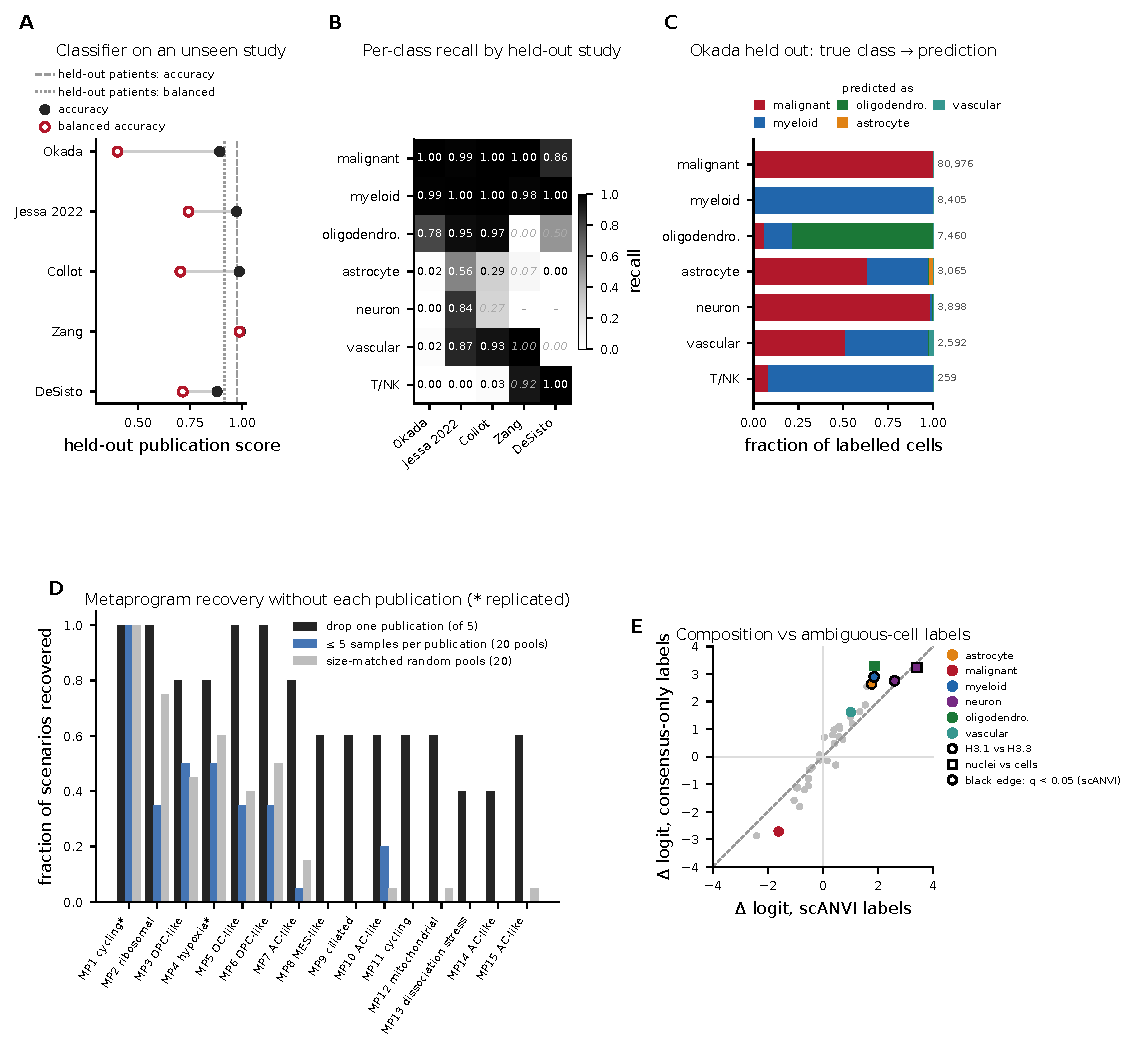
\includegraphics[width=\textwidth]{fig7_robustness.pdf}
\caption{\textbf{Robustness of the reference to removing one study.} \textbf{a}, Accuracy and balanced accuracy on each
held-out publication after retraining scVI and scANVI without it; dashed and dotted lines mark the held-out-patient
accuracy and balanced accuracy of the released model. \textbf{b}, Per-class recall for each held-out publication; grey
italic values are based on fewer than 20 cells. \textbf{c}, Predicted labels for each true class of the post-mortem
series when that series is held out. \textbf{d}, Fraction of scenarios in which each metaprogram is recovered (gene-set
Jaccard similarity $\geq 0.5$); asterisks mark the two replicated metaprograms. \textbf{e}, Composition coefficients
under scANVI labels against consensus-only labels; coloured points are significant ($q < 0.05$) under at least one
labelling, with a black edge when significant under scANVI labels.}
\label{fig:robust}
\end{figure}

% ================= DISCUSSION =================
\section{Discussion}

We present a reference of H3 K27-altered DMG built from 52 patients, with harmonised labels, calibrated malignant calls
and reference models whose performance on new patients and on new studies has been measured. Because individual DMG
cohorts contain few patients, this reference allows patient-level questions that no single public dataset can address.

Most of our findings define the limits of what public DMG data can establish. Only cycling and hypoxia replicated under a
rule specified in advance, and of these only cycling was recovered in every robustness scenario. Lineage-like programmes were
detected only in nuclei, and this did not change when 22 whole-cell Smart-seq2 samples were added: whole-cell cohorts
yielded their own astrocyte-like programme, with different gene content. Lineage programmes therefore depend on platform
and cohort as well as on assay, and matched whole-cell and nucleus data from the same tumours are needed to resolve
them. By contrast, the ciliated programme carries the tumour's copy-number profile, which identifies it as a tumour state;
in the data of Jessa et al.\ \citep{jessa2022km}, 10\% of the cells with this programme had been annotated as ependymal by
the original authors.
This mirrors pan-cancer evidence that recurrent programmes are identified reliably only across many tumours
\citep{gavish2023hallmarks}, and adds that recurrence across cohorts is insufficient when cohorts differ systematically
in sample preparation. Similarly, the H3.1--H3.3 difference in neuron abundance and the differences between cells and
nuclei are confounded with study by design.

The leave-one-study-out analysis has a practical implication for tumour reference atlases. Accuracy on held-out patients,
a commonly reported measure, overstated performance on a new study
(balanced accuracy 0.917 versus 0.506). A reference composed mainly of tumour tissue transferred malignant and myeloid
identities reliably but classified unfamiliar normal cells as malignant, with high confidence. We therefore recommend
leave-one-study-out evaluation for tumour references, and copy-number or marker evidence to support normal-lineage calls
in new data.

The weak co-localisation of MES-like tumour cells with myeloid and vascular cells is consistent with the hypoxia-associated
mesenchymal compartment described in glioblastoma \citep{neftel2019integrative} and with bone morphogenetic protein
(BMP)-driven invasive phenotypes in DMG \citep{huchede2024bmp}. The brainstem gradient is consistent with an infiltrative
tumour front but rests on a single autopsy. Engineered brainstem organoid models of H3.3K27M DMG \citep{bessler2026de}
provide a means to test these associations experimentally.

\subsection{Limitations}

This study has several limitations. One post-mortem series contributes half of the cells and every autopsy sample, so
autopsy and resection cannot be compared. All H3.1 samples are pontine nuclei, and the H3 variant is unreported for 25
of 57 samples. Whole-cell data for programme discovery come from few cohorts and two platforms. Per-cell
metaprogram-family labels, and the spatial reference built from them, reflect relative programme activity within a sample
rather than abundance. The reference lacks normal progenitor
and ependymal classes, and on unseen studies the classifier often misclassifies rare normal lineages as malignant.
Copy-number thresholds were tuned on 22 samples, and 11.2\% of consensus-malignant reference cells rely on the
aggregate copy-number score without a supporting arm-level event. In 21 of 50 samples the selected NMF rank was the
largest tested ($k = 9$); extending the range to $k = 12$ changed the rank of 14 samples but not the conclusions (see
Results). The spatial conclusions are based on 12 patients with high between-patient
heterogeneity. Finally, two query cohorts were deposited without raw counts.

% ================= METHODS =================
\section{Methods}

\subsection{Data collection}
In October 2026 we screened GEO series (78 candidate series in two searches) and the OpenAlex literature database (393
records) for human DMG data generated by single-cell or single-nucleus RNA sequencing or Visium spatial transcriptomics.
Data sets were included if they contained primary human H3 K27-altered midline glioma or normal human brain tissue and
provided processed expression matrices; reasons for exclusion are listed in Supplementary Table~\ref{tab:deposits}. The
reference comprised GEO GSE210567 and GSE210566 \citep{jessa2022km}, Zenodo 10.5281/zenodo.17922773
\citep{collot2026igsfvista}, GSE231859 \citep{desisto2024tumor}, GSE245674 (sample GSM7846769) \citep{zang2024singlecell}
and the post-mortem series of \citet{okada2026singlenucleus} (processed matrix from its UCSC Cell Browser instance; raw
reads under controlled access at the European Genome-phenome Archive, EGAS50000001447). Projection-only cohorts were
GSE102130 \citep{filbin2018developmental}, GSE184357 \citep{liu2022landscape}, GSE227983 and GSE271936, and two normal brain
references obtained from CZ CELLxGENE Discover \citep{abdulla2025czcellxgene}: the hindbrain, pons and medulla dissections
of a first-trimester brain atlas \citep{braun2023comprehensive}, of which 100,000 cells were sampled, and six adult pons
dissections \citep{siletti2023transcriptomic}, of which 100,000 nuclei were sampled. Spatial cohorts were GSE268577
\citep{huchede2024bmp}, GSE194329 \citep{ren2023spatial}, GSE280990 \citep{kordowski2025spatial} and Zenodo 10.5281/zenodo.17922773. All data were
human and previously published, and each study obtained its own ethical approval and informed consent.

\subsection{Gene harmonisation and quality control}
Gene identifiers were mapped to the GENCODE v32 annotation of the 10x Genomics GRCh38-2020-A reference, by Ensembl
identifier where available and otherwise by exact symbol or unique alias; ambiguous symbols were removed and duplicated
genes were summed. The reference used the 18,882 genes measured in every sample of every UMI study. Quality control was
applied per assay class with Scanpy \citep{wolf2018scanpy}. Nuclei were retained with at least 300 detected genes and a
mitochondrial read fraction of at most 5\% (20\% for four nucleus samples with cytoplasmic contamination); whole cells with
at least 300 genes and at most 20\% mitochondrial reads; and Smart-seq2 profiles with at least 1,000 genes and at most 20\%
mitochondrial reads (5\% for Smart-seq2 profiles of frozen nuclei).
Cells above the 99.5th percentile of detected genes within their sample were removed. Doublets were scored per sample with
Scrublet \citep{wolock2019scrublet} (expected doublet rate 0.06, 3,000 highly variable genes), and cells with a score above
0.25 were removed from the reference. Samples whose retained cells had a median of fewer than 500 detected genes were
flagged as low confidence.

\subsection{Malignant-cell calling}
Counts were normalised to 10,000 per cell and log-transformed, and each cell was scored with the Scanpy gene-set scoring function
against marker sets for myeloid cells (\textit{PTPRC}, \textit{CSF1R}, \textit{CX3CR1}, \textit{P2RY12}, \textit{C1QA},
\textit{C1QB}, \textit{CD74}), T and natural killer cells (\textit{CD3D}, \textit{CD3E}, \textit{CD2}, \textit{NKG7}),
oligodendrocytes (\textit{MBP}, \textit{PLP1}, \textit{MOG}, \textit{MAG}, \textit{ST18}), vascular cells
(\textit{CLDN5}, \textit{FLT1}, \textit{VWF}, \textit{PDGFRB}, \textit{RGS5}), neurons (\textit{RBFOX3}, \textit{SYT1},
\textit{SNAP25}, \textit{GAD1}, \textit{SLC17A7}), astrocytes (\textit{AQP4}, \textit{GFAP}) and the OPC-like
(\textit{PDGFRA}, \textit{OLIG1}, \textit{OLIG2}, \textit{SOX10}, \textit{CSPG4}), AC-like (\textit{GFAP}, \textit{AQP4},
\textit{APOE}, \textit{CLU}), MES-like (\textit{CD44}, \textit{VIM}, \textit{CHI3L1}, \textit{ANXA1}) and cycling
(\textit{MKI67}, \textit{TOP2A}) tumour states. A cell was called normal by markers if its best normal-lineage score was at
least 0.25, exceeded the best competing tumour-state score by at least 0.10 and exceeded the astrocyte score; normal cells
with a score of at least 0.50 and at least twice the second-best lineage score served as copy-number references.

Copy-number profiles were computed per sample in the manner of inferCNV, using autosomal genes expressed in at least
10\% of cells and ordered by GENCODE v32 coordinates \citep{frankish2023gencode}. For each cell, log-normalised expression
was compared with the mean of each reference lineage, clipped at $\pm 3$, smoothed as a running mean over 100-gene windows
with a step of 10 genes and median-centred, and the lineage with the smallest mean absolute deviation was retained as the
baseline. Values below 1.5 standard deviations of the sample were set to zero. Profiles were computed within each
chromosome and, for arm-level events, within each chromosome arm; the copy-number score of a cell was its mean absolute
smoothed deviation. The reference for each sample combined its own immune cells with up to 300 myeloid and T or
natural killer cells pooled from other samples of the same study and assay, and with up to 300 oligodendrocyte, vascular and
neuronal cells per lineage pooled from other samples after removal of cells in tumour-grade copy-number clusters; a sample's
own non-immune cells were never used as reference. Reference cells with a copy-number score above the reference median plus
three median absolute deviations were removed, and samples with fewer than 30 reference cells were not called. Cells were clustered by the Leiden algorithm (resolution 1.0) on principal components of the copy-number profile.
A cluster was called malignant if its mean copy-number score exceeded the reference mean by 0.008, if one recurrent arm-level
event (gain of 1q, 2 or 7; loss of 10q, 13q, 14q or 17p) reached $z \geq 2$ relative to the reference, or if two events
reached $z \geq 1$; clusters containing at least 20\% reference cells additionally required both score elevation and an
event. The consensus call was malignant or normal when the marker and copy-number calls agreed (and, where available, the
author label agreed), and ambiguous otherwise. The permissive variant additionally called malignant those marker-normal
cells that lay in a malignant cluster with a supporting arm-level event and had no contradicting author label. Agreement
with author labels was computed per sample.

\subsection{Integration}
Of the shared genes, 3,000 highly variable genes were selected with the Seurat v3 method using sample as batch
\citep{stuart2019comprehensive}. scVI \citep{lopez2018deep} was trained on raw counts with sample as the batch variable,
study and assay as categorical covariates and mitochondrial fraction as a continuous covariate (30 latent dimensions, two
hidden layers, negative binomial likelihood, batch size 1,024, at most 26 epochs with early stopping on the evidence lower
bound of a random 10\% validation set, patience 5), with random seeds 0, 1 and 2. Integration was scored with scib-metrics
\citep{luecken2021benchmarking} on 60,023 labelled cells subsampled by sample, using a 90-nearest-neighbour graph: iLISI,
kBET, batch average silhouette width and principal component regression for each batch variable (sample, study and assay)
and graph connectivity for batch correction; and cLISI, label silhouette width, normalised mutual information and adjusted
Rand index for biological conservation. Each metric was min--max scaled across the evaluated embeddings, and the score
0.4 $\times$ batch + 0.6 $\times$ biology, specified in advance, selected among the scVI seeds; Harmony
\citep{korsunsky2019fast} and uncorrected principal components served as benchmarks. Uniform manifold approximation and
projection (UMAP) was used for visualisation only \citep{becht2018dimensionality}.

\subsection{Label transfer and query mapping}
scANVI \citep{xu2021probabilistic} was initialised from the selected scVI model with the consensus lineage labels (ambiguous
cells unlabelled) and trained on all labelled cells for at most 25 epochs. Early stopping (patience 5) monitored the
classification loss on a validation set of whole patients, comprising about 10\% of labelled cells and containing every
class, and the weights of the best epoch were restored. Query cohorts were restricted to the 3,000 reference genes and
encoded by the reference model without further training. For the two cohorts deposited as TPM (Filbin et al.\ and
LaBelle et al.), pseudo-counts were derived by rescaling each cell's TPM values so that their sum equalled the number of
detected genes multiplied by the median counts per detected gene of a matching count-based cohort (Liu et al.\ RSEM
counts for Smart-seq2 data and Jessa et al.\ 10x data for 10x data), and rounding; Liu et al.\ expected counts were
rounded. These cohorts were used for projection only. Labels were transferred by the scANVI classifier and by a
majority vote of the 15 nearest reference cells in the latent space. Mapping uncertainty was the mean distance of a query
cell to its 15 nearest reference cells, expressed as a percentile of the same quantity among 50,000 reference cells
\citep{lotfollahi2021mapping}.

\subsection{Metaprograms}
Malignant cells were those with a consensus call of malignant that passed quality control. For each sample with at least
200 such cells, genes detected in at least three cells were reduced to 2,000 highly variable genes (Seurat v3), normalised
to 10,000 counts per cell and log-transformed. Non-negative matrix factorisation (scikit-learn; random initialisation,
coordinate descent, 500 iterations) was run with ten random restarts for each rank $k$ from 4 to 9; components were
clustered by average linkage on cosine distance, and the consensus programme was the median of each cluster
\citep{kotliar2019identifying}. The selected rank was the largest $k$ whose clustering had a silhouette of at least 0.90 and
whose clusters each contained components from at least 80\% of restarts. Each programme was represented by its 50 genes
with the highest gene spectra scores. Programmes from all samples were clustered by average linkage on Jaccard distance;
at a cut of 0.85, clusters containing at least five programmes from at least three samples were metaprograms, each
represented by up to 50 genes present in at least 25\% of its member programmes. A metaprogram replicated if its member
programmes came from at least three publications and from both cells and nuclei; the two Jessa et al.\ series counted as
one publication. The cut and the rule were specified before inspection of the results. Metaprograms were labelled by the
reference gene set with the largest significant overlap (hypergeometric test, Benjamini--Hochberg $q < 0.05$, at least five
shared genes), and metaprograms whose 50 genes included at least 15 ribosomal-protein genes, at least 5 mitochondrial genes, or at
least 10 genes of a curated immediate-early and heat-shock set were classified as technical.

For the masking control, malignant-cell counts of each Jessa et al.\ sample were summed into pseudobulk profiles (log$_2$
counts per million). A gene was assay-biased if it differed by at least two-fold in the same direction in both patients
profiled as both cells and nuclei, and differed in that direction between the 4 cell and 23 nucleus samples (Welch $t$-test,
Benjamini--Hochberg $q < 0.05$); mitochondrial and ribosomal-protein genes were added. The 6,013 assay-biased genes were
removed from each programme before re-clustering, and the result was compared with ten random masks that removed the same
number of genes from each programme.

Per-cell metaprogram families were assigned by scoring each metaprogram with UCell \citep{andreatta2021ucell} (maximum rank 1,500), standardising
scores within sample, averaging the standardised scores of the metaprograms in each family, and taking the family with the
highest positive score. Technical metaprograms, and metaprograms whose median UCell score in normal myeloid or vascular cells
was at least twice that in malignant cells, were excluded from the families. Cells with a highest family score of at least
1 were used to build the spatial reference.

\subsection{Microenvironment subclustering}
Cells passing quality control and not called malignant were assigned to a compartment (myeloid, T and natural killer,
vascular or oligodendroglial) by their consensus lineage label or, for ambiguous cells, by a scANVI label with probability
of at least 0.9. Each compartment was clustered by the Leiden algorithm (resolution 0.5) on a 15-nearest-neighbour graph
of the scVI latent space. Except in the T and natural killer compartment, subclusters with fewer than 50 cells, or whose
mean marker score for another lineage exceeded that for their own, were removed. For the remaining cells, a
separate scVI model was trained per compartment on 2,000 highly variable genes after removal of assay-biased,
mitochondrial and ribosomal genes (20 latent dimensions, assay class as a covariate, at most 400 epochs with early stopping,
patience 20), and cells were re-clustered (Leiden, resolution 0.5). Subclusters were annotated by the reference marker set
with the highest mean score and characterised by Wilcoxon rank-sum tests against the other subclusters of the compartment.
Assay purity was the fraction of cells in subclusters with less than 10\% or more than 90\% nuclei.

\subsection{Composition models}
Four composition sets were modelled: lineages of all cells passing quality control (scANVI labels); malignant states
(OPC-like, AC-like, OC-like, MES-like and cycling, assigned by the highest within-sample standardised gene-set score);
metaprogram families (standardised within assay class); and microenvironment subclusters within each compartment
(samples with at least 30 cells). The contrasts were thalamus versus pons, adult versus paediatric, H3.1 versus H3.3,
dordaviprone (ONC201) with standard care versus standard care alone, autopsy versus resection, and nuclei versus cells;
samples with unknown or other levels were excluded from each contrast. For each sample with at least 200 cells (lineages,
states and families), the proportion of each category was transformed to an empirical logit,
$\log\{(k + 0.5)/(n - k + 0.5)\}$, where $k$ is the number of cells in the category and $n$ the number in the sample. Each
contrast was modelled by ordinary least squares with publication as a fixed effect, adjusting for assay class where it
varied within a publication, and with standard errors clustered by patient. Contrasts without variation within any
publication were not estimated. The H3-variant contrast was refitted with site as a covariate and within pontine samples.
$P$ values were corrected by the Benjamini--Hochberg method \citep{benjamini1995controlling} within each contrast.

\subsection{Spatial deconvolution and statistics}
In-tissue spots from Space Ranger filtered matrices were used, with genes restricted per cohort to those present in every
section and in the reference. Reference signatures for cell2location \citep{kleshchevnikov2022celllocation} were estimated
from 59,993 cells in 13 classes (seven malignant metaprogram families and six normal lineages; at most 8,000 cells per class,
sampled within class by sample) with a negative binomial regression model (250 epochs, sample as batch). Each cohort was
deconvolved with an expected 5 cells per spot and a detection alpha of 20, for between 2,000 and 20,000 epochs set by a fixed
GPU time budget; the realised number of epochs was recorded. Spot proportions were the 5\% posterior quantile of each class
divided by their sum over classes. Co-localisation between each of 7 malignant families and 6 normal lineages (42 pairs) was
measured as the Spearman correlation of spot proportions per section, Fisher $z$-transformed, averaged within patient,
pooled across patients by DerSimonian--Laird random effects \citep{dersimonian1986meta}, and corrected by the
Benjamini--Hochberg method. The ten sections from one autopsy were treated as one patient. Spots with fewer
than 500 UMIs were removed in a sensitivity analysis. As a further sensitivity analysis, correlations were
recomputed on centred log-ratio-transformed proportions.

\subsection{Robustness analyses}
For each of the five publications, scVI was retrained without it using the settings of the released model (seed 1), and
scANVI was trained from it with early stopping on a patient-grouped validation set drawn only from the remaining
publications. The held-out publication was then mapped by scArches surgery \citep{lotfollahi2021mapping} with default
parameter freezing, no weight decay and 100 epochs, with its labels hidden and used only for scoring. Balanced accuracy was
the mean recall over classes with at least 20 cells in the held-out publication. Metaprograms were re-clustered with the
unchanged rule after removing each publication, in 20 pools of at most five samples per publication, and in 20 random pools
of equal size; a primary metaprogram was recovered when a metaprogram in the scenario had a gene-set Jaccard similarity of at
least 0.5 with it. Re-clustering of all samples reproduced the primary result exactly. Composition models were refitted
under four labellings of ambiguous cells, after confirming that the original labelling reproduced the published
coefficients.

For the whole-cell extension, malignant cells (consensus call malignant, passing quality control) of Liu et al.\ (RSEM
expected counts, rounded) and Filbin et al.\ (TPM, rounded) were factorised per sample with the procedure above, using a
minimum of 100 malignant cells per sample because Smart-seq2 detects more genes per cell than droplet methods; Liu et al.\
samples prepared from frozen nuclei were classed as nuclei. Their programmes were clustered with the primary programmes
using the unchanged rule. For the MP9 analysis, cells with a within-sample standardised MP9 score of at least 2 were
compared with the sample's other malignant cells and its normal reference cells on the seven arm-level copy-number values:
the tumour index projected each cell onto the axis from the normal-reference mean to the mean of the other malignant cells
(0, normal; 1, other malignant), in samples with at least 20 MP9-high and 30 reference cells. Spatial correlations were
re-pooled with Hartung--Knapp--Sidik--Jonkman intervals ($t$ distribution with $k - 1$ degrees of freedom across patients),
and signature similarity was the cosine similarity of gene-centred log-transformed cell2location signatures. For the rank extension, samples that had selected $k = 9$ were re-factorised
for $k = 10$--$12$ with the same restarts and selection rule, and their programmes were replaced when a larger rank
qualified. The
composition test of family assignments used the area under the receiver operating characteristic curve of the per-sample
family fraction for samples with versus without a programme of that family.

\subsection{Statistics and reproducibility}
Patients were the unit of inference for tumour-level claims. Multiple testing was controlled by the Benjamini--Hochberg method within each family of tests, as described above.
All analyses were scripted with fixed random seeds and record checksums of their inputs. Software versions are listed in
Supplementary Table~\ref{tab:keyresources}.

% ================= BACK MATTER =================
\section{Data availability}
The atlas data and reference models are available at Zenodo
(\href{https://doi.org/10.5281/zenodo.23623335}{doi:10.5281/zenodo.23623335}).

\section{Code availability}
All analysis code and documentation are available at \url{https://github.com/hossainlab/dmg_atlas}.

\section{Acknowledgements}
We thank the investigators and patients of every cohort reused here.

\section{Author contributions}
M.J.H. conceived the study, performed all analyses and wrote the manuscript. I.M. mentored the project.

\section{Competing interests}
The authors declare no competing interests.

\section{Use of AI-assisted technologies}
The authors used Claude (Anthropic) to assist with analysis code, documentation and
drafting. The authors reviewed and edited all content and take full responsibility for it.

\section{Supplementary information}
Supplementary Figs.~\ref{sfig:1}--\ref{sfig:7} and Supplementary Tables~\ref{tab:deposits}--\ref{tab:keyresources} follow
the references; Supplementary Data~1--6 are provided as separate Excel files.

\bibliography{references}

% ================= SUPPLEMENTARY INFORMATION =================
\clearpage
\nolinenumbers
\singlespacing
\section{Supplementary Information}
\setcounter{figure}{0}\setcounter{table}{0}
\captionsetup[figure]{name=Supplementary Fig.}
\captionsetup[table]{name=Supplementary Table}

\subsection{Supplementary Figures}
\begin{figure}[htbp]\centering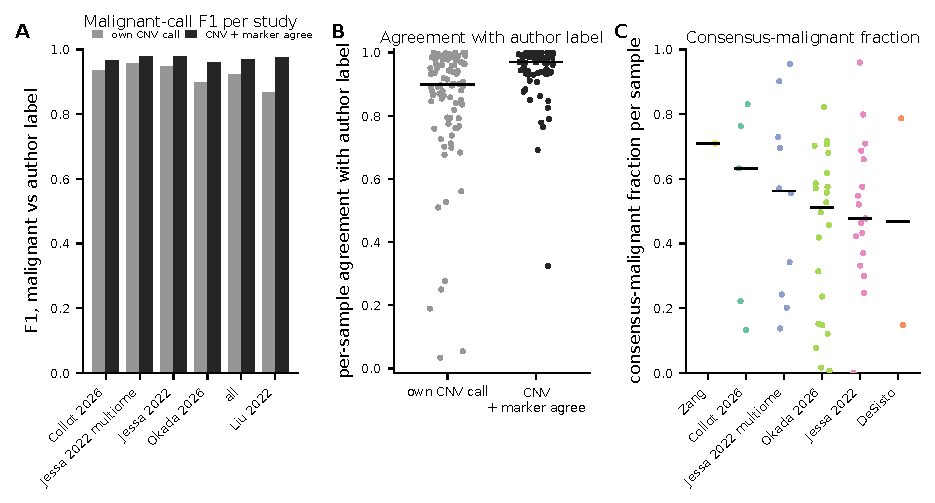
\includegraphics[width=0.95\textwidth]{figS1_malignant_calls.pdf}
\caption{\textbf{Malignant-cell calls.} \textbf{a}, F1 of the author-independent malignant calls against author labels per
study: own copy-number call, and cells where copy-number and marker calls agree. \textbf{b}, Per-sample agreement with
author labels (samples with at least 100 compared cells). \textbf{c}, Fraction of consensus-malignant cells per reference
sample, by study.}\label{sfig:1}\end{figure}

\begin{figure}[htbp]\centering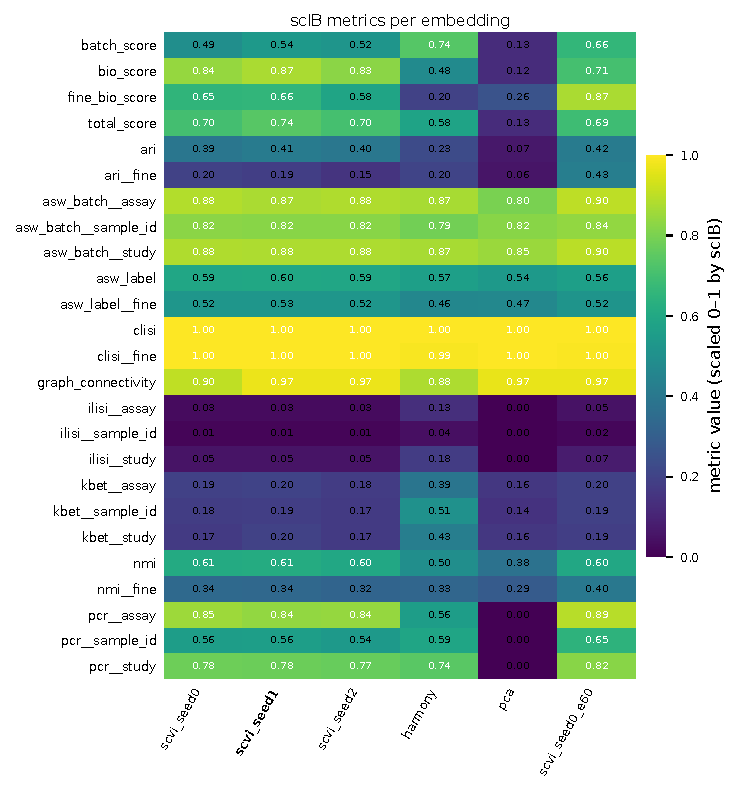
\includegraphics[width=0.95\textwidth]{figS2_integration_metrics.pdf}
\caption{\textbf{Integration benchmark.} Batch-correction metrics (batch keys sample, study, assay) and
biological-conservation metrics (coarse and fine labels) for the six candidate embeddings, with summary scores above.
Assay remains the hardest batch key for the chosen model.}\label{sfig:2}\end{figure}

\begin{figure}[htbp]\centering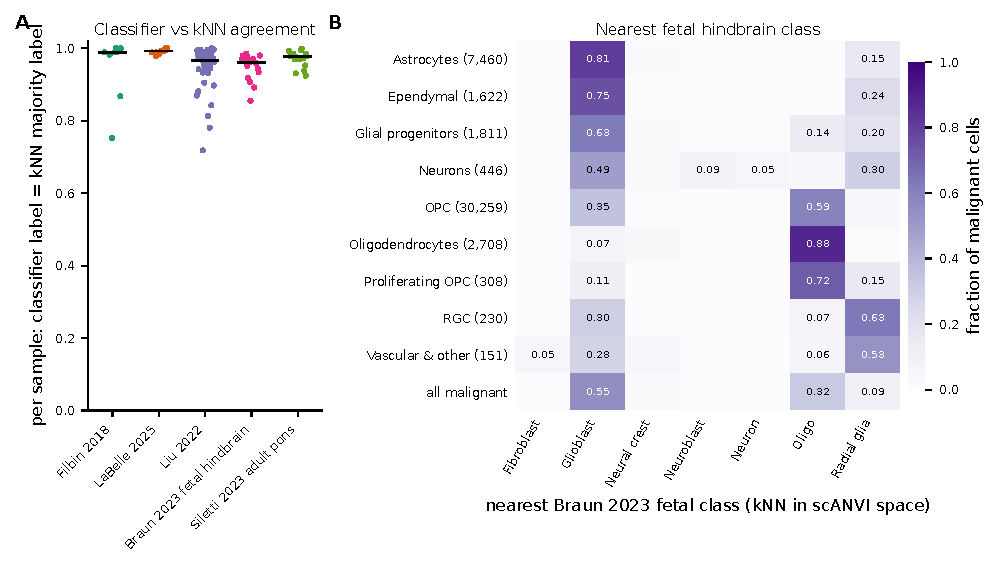
\includegraphics[width=0.95\textwidth]{figS3_mapping_origin.pdf}
\caption{\textbf{Mapping confidence and nearest fetal class.} \textbf{a}, Per-sample fraction of query cells whose
classifier label equals the majority label of their 15 nearest reference cells. \textbf{b}, Nearest fetal hindbrain class
of malignant cells, overall and by author state.}\label{sfig:3}\end{figure}

\begin{figure}[htbp]\centering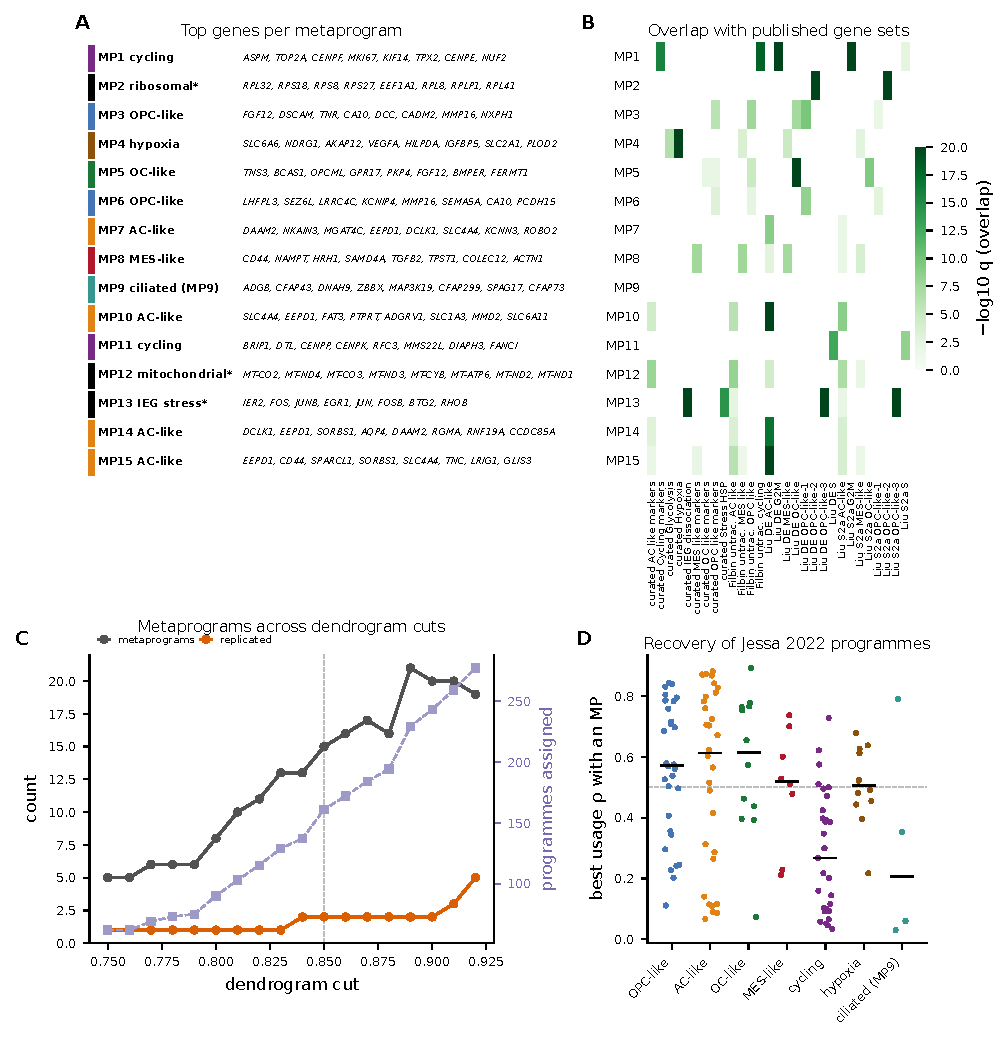
\includegraphics[width=0.95\textwidth]{figS4_metaprogram_detail.pdf}
\caption{\textbf{Metaprogram content and robustness.} \textbf{a}, Top eight genes of each metaprogram; asterisk, technical
programme. \textbf{b}, Overlap of metaprogram top-50 genes with published DMG and glioma state gene sets (hypergeometric
test, Benjamini--Hochberg $q$). \textbf{c}, Metaprograms, replicated metaprograms and assigned programmes across dendrogram
cuts. \textbf{d}, Best within-sample correlation of published per-sample programmes with an atlas metaprogram.}\label{sfig:4}\end{figure}

\begin{figure}[htbp]\centering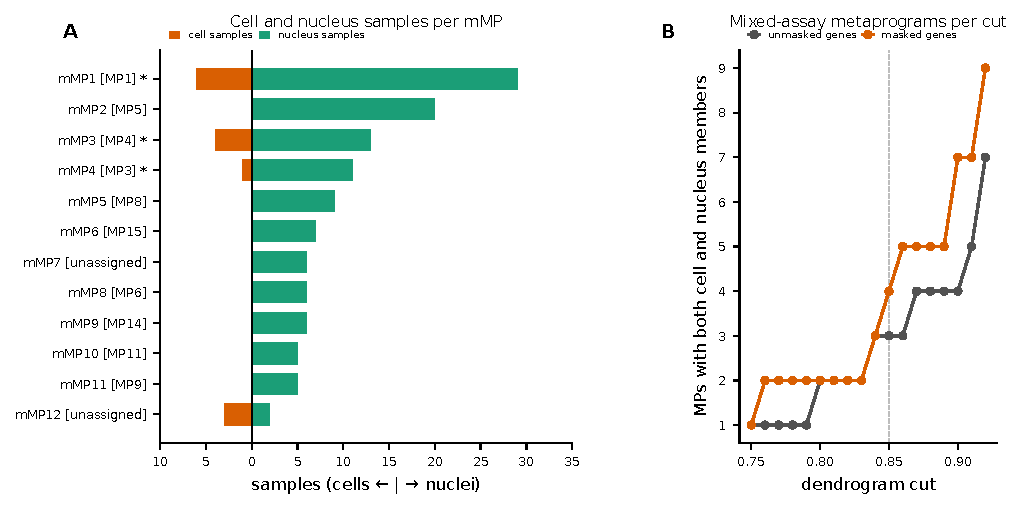
\includegraphics[width=0.95\textwidth]{figS5_masked_metaprograms.pdf}
\caption{\textbf{Metaprograms after masking assay-biased genes.} \textbf{a}, The 12 masked metaprograms at the primary cut,
with contributing cell and nucleus samples. \textbf{b}, Metaprograms containing both cell- and nucleus-derived programmes
across cuts, with all genes and after masking.}\label{sfig:5}\end{figure}

\begin{figure}[htbp]\centering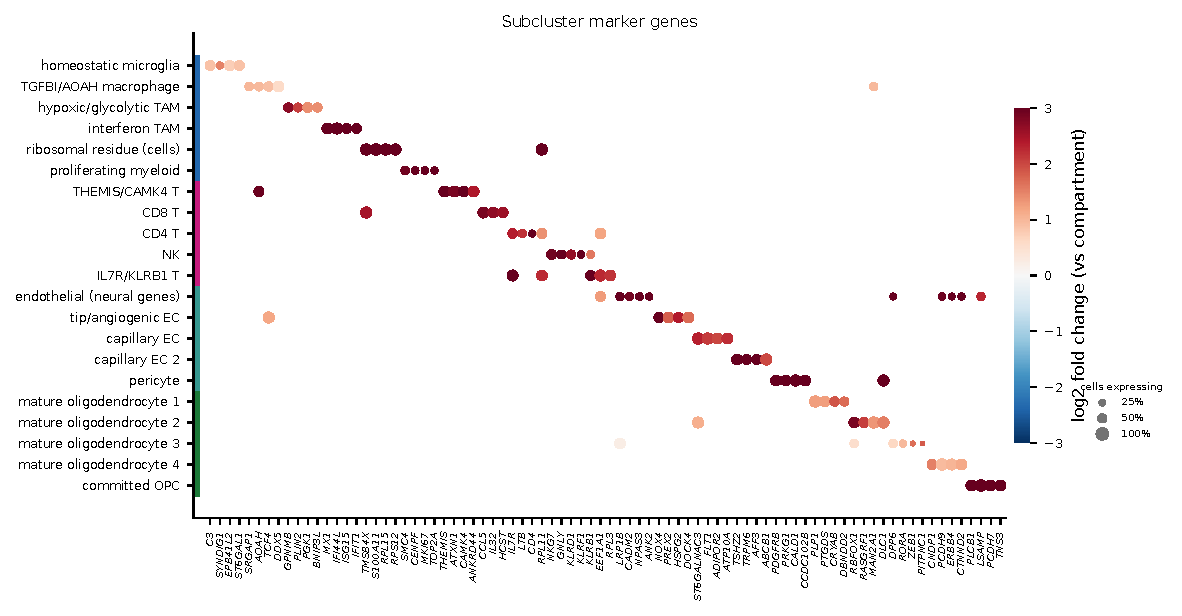
\includegraphics[width=0.95\textwidth]{figS6_tme_markers.pdf}
\caption{\textbf{Marker genes of the microenvironment subclusters.} Top four genes per subcluster; dot size, fraction of
the subcluster's cells expressing the gene; colour, log fold change against the other subclusters of the same
compartment.}\label{sfig:6}\end{figure}

\begin{figure}[htbp]\centering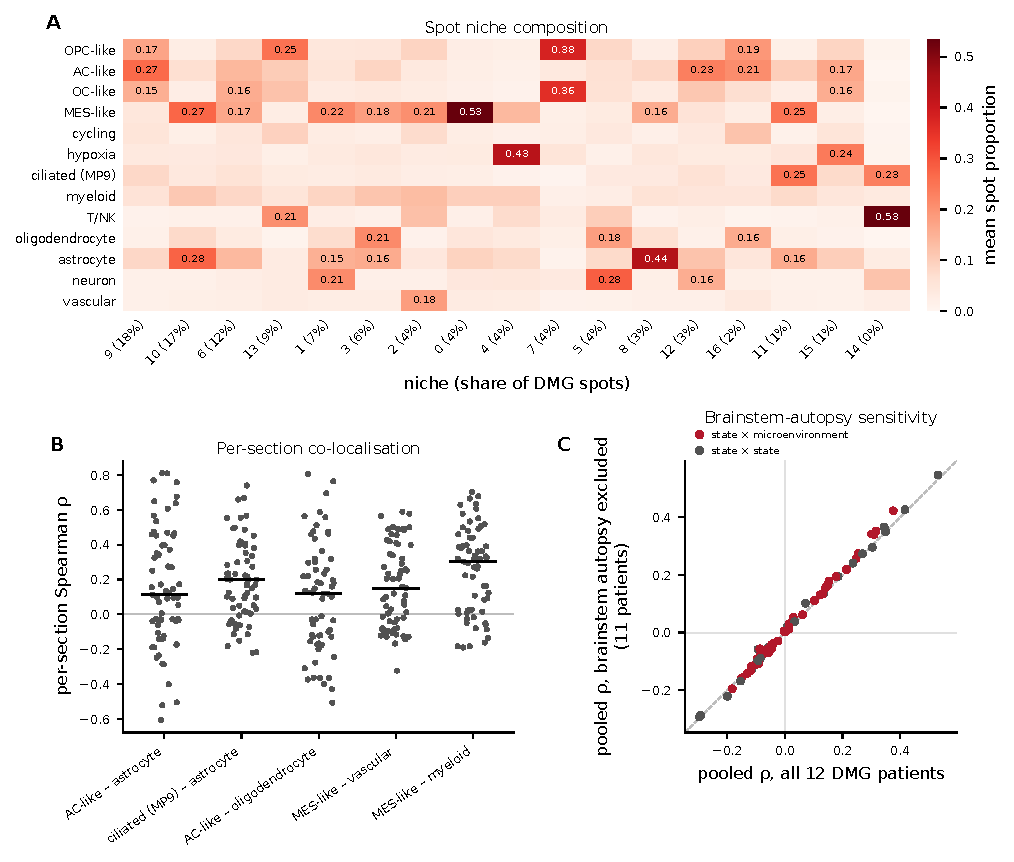
\includegraphics[width=0.95\textwidth]{figS7_spatial_detail.pdf}
\caption{\textbf{Spatial niches and sensitivity analyses.} \textbf{a}, Mean class proportions of the 16 spot niches.
\textbf{b}, Per-section correlations for the six strongest pairs of Fig.~\ref{fig:spatial}d, computed with three
metrics (proportion, centred log-ratio and abundance); each point is one section and metric, and ten sections come from one
autopsy. \textbf{c}, Pooled correlations with and without that autopsy.}\label{sfig:7}\end{figure}

\clearpage
\begin{landscape}
\footnotesize
\setlength{\tabcolsep}{4pt}\renewcommand{\arraystretch}{1.05}
\begin{longtable}{>{\raggedright\arraybackslash}p{6.2cm}>{\raggedright\arraybackslash}p{6.0cm}>{\raggedright\arraybackslash}p{3.2cm}>{\raggedright\arraybackslash}p{3.4cm}>{\raggedright\arraybackslash}p{4.6cm}}
\caption{\textbf{Public data sets screened and their use in this study.} Data sets used, with their role, followed by data
sets screened but not used, with the reason.}
\label{tab:deposits}\\
\toprule
Data set & Accession & Repository & Data type & Use in this study \\
\midrule
\endfirsthead
\toprule
Data set & Accession & Repository & Data type & Use in this study \\
\midrule
\endhead
Collot et al., DMG & 10.5281/zenodo.17922773 & Zenodo & snRNA-seq & Reference \\
DeSisto et al., paediatric HGG & GSE231859 & GEO & scRNA-seq & Reference \\
Jessa et al., DMG & GSE210566 & GEO & Multiome (RNA) & Reference \\
Jessa et al., DMG & GSE210567 & GEO & scRNA-seq, snRNA-seq & Reference \\
Okada et al., post-mortem DMG & UCSC Cell Browser (brain-dmg-multiomics); raw data EGAS50000001447 & EGA / UCSC Cell Browser & snRNA-seq & Reference \\
Zang et al., DMG & GSE245674 (GSM7846769) & GEO & scRNA-seq & Reference \\
Braun et al., first-trimester human brain & CELLxGENE collection 4d8fed08 & CZ CELLxGENE & scRNA-seq & Query (normal brain) \\
Filbin et al., H3K27M glioma & GSE102130 & GEO & Smart-seq2 (TPM) & Query (tumour) \\
LaBelle et al., DMG immune cohort & GSE227983, GSE271936 & GEO & Smart-seq2, 10x (TPM) & Query (tumour) \\
Liu et al., H3-K27M DMG & GSE184357 & GEO & Smart-seq2 (TPM) & Query (tumour) \\
Siletti et al., adult human brain & CELLxGENE collection 283d65eb & CZ CELLxGENE & snRNA-seq & Query (normal brain) \\
Whole-brainstem DIPG autopsy Visium & GSE280990 & GEO & Visium & Spatial \\
Collot et al., DMG Visium & 10.5281/zenodo.17922773 & Zenodo & Visium & Spatial \\
Huchede et al., DMG Visium & GSE268577 & GEO & Visium & Spatial \\
Ren et al., DMG and glioblastoma Visium & GSE194329 & GEO & Visium & Spatial \\
\midrule
Adult human brain Paired-Tag (Xie et al.) & GSE327101 & GEO & Paired-Tag & Not used: normal reference not required \\
PBTA / OpenPedCan v14 & -- & OpenPedCan & Bulk RNA-seq & Not used: bulk data, outside scope \\
ScPCA SCPCP000021 & SCPCP000021 & ScPCA portal & snRNA-seq & Excluded: failed quality control \\
Mouse developing pons and forebrain (Jessa et al.) & GSE188625 & GEO & scRNA-seq (mouse) & Excluded: non-human \\
Longitudinal paediatric high-grade glioma & -- & dbGaP & snRNA-seq, snATAC-seq & Not accessed: controlled access \\
DIPG CAR-T autopsy cohort & -- & -- & snRNA-seq & Not available: data not released \\
DIPG single-cell cohort (2026) & -- & EGA & scRNA-seq & Not available: not deposited \\
Cell-line and PDX series & GSE212782 and others & GEO & scRNA-seq & Excluded: models, not primary tumour \\
CSF and PBMC immune series & GSE261235, GSE186802, GSE202174 & GEO & scRNA-seq & Excluded: not tumour tissue \\
\bottomrule
\end{longtable}
\end{landscape}


\clearpage
\begin{table}[htbp]
\centering\scriptsize
\caption{\textbf{Key resources table.} Deposited data reused in this study and the software that produced the
results. Version numbers are those recorded by \texttt{scripts/28\_record\_environment.py}; the full environment
(557 conda and 167 pip entries for the local environment, plus the GPU image pins) is in \texttt{env/}.}
\label{tab:keyresources}
\setlength{\tabcolsep}{3pt}
\begin{tabular}{p{5.0cm}p{6.0cm}p{3.6cm}}
\toprule
\multicolumn{3}{l}{\textbf{Deposited data}} \\
Dataset & Identifier & Source \\
\midrule
Collot et al., DMG (snRNA) & Zenodo: 10.5281/zenodo.17922773 (scRNA.tar.gz) & Zenodo \\
DeSisto et al., paediatric HGG (scRNA) & GSE231859 & GEO \\
Jessa et al., DMG (multiome RNA) & GSE210566 & GEO \\
Jessa et al., DMG (sc/snRNA) & GSE210567 & GEO \\
Okada et al., post-mortem DMG (snRNA) & EGAS50000001447 (raw, controlled); processed matrix from the study's UCSC Cell Browser instance & EGA / UCSC Cell Browser \\
Zang et al., DMG (scRNA) & GSE245674 (GSM7846769) & GEO \\
Braun et al., first-trimester human brain & CZ CELLxGENE Discover (collection 4d8fed08-2d6d-4692-b5ea-464f1d072077) & CZ CELLxGENE \\
Filbin et al., H3K27M glioma (Smart-seq2, TPM) & GSE102130 & GEO \\
DMG immune cohort (SS2 + 10x, TPM) & GSE227983 & GEO \\
Liu et al., H3-K27M DMG (Smart-seq2, TPM) & GSE184357 & GEO \\
Siletti et al., adult human brain (pons dissections) & CZ CELLxGENE Discover (collection 283d65eb-dd53-496d-adb7-7570c7caa443) & CZ CELLxGENE \\
Whole-brainstem DIPG autopsy Visium & GSE280990 & GEO \\
Collot et al., DMG Visium & Zenodo: 10.5281/zenodo.17922773 (ST.tar.gz) & Zenodo \\
Huchede et al., DMG Visium & GSE268577 & GEO \\
Ren et al., DMG and glioblastoma Visium & GSE194329 & GEO \\
\midrule
\multicolumn{3}{l}{\textbf{Software and algorithms}} \\
Software & Reference & Identifier \\
\midrule
python v3.11.16 & Python Software Foundation & \url{https://pypi.org/project/python/} \\
numpy v2.4.6 & Harris et al. & \url{https://pypi.org/project/numpy/} \\
scipy v1.17.1 & Virtanen et al. & \url{https://pypi.org/project/scipy/} \\
pandas v2.3.3 & McKinney & \url{https://pypi.org/project/pandas/} \\
anndata v0.12.19 & Virshup et al. & \url{https://pypi.org/project/anndata/} \\
scanpy v1.11.5 & Wolf et al. & \url{https://pypi.org/project/scanpy/} \\
scikit-learn v1.7.2 & Pedregosa et al. & \url{https://pypi.org/project/scikit-learn/} \\
statsmodels v0.15.0 & Seabold and Perktold & \url{https://pypi.org/project/statsmodels/} \\
matplotlib v3.11.2 & Hunter & \url{https://pypi.org/project/matplotlib/} \\
infercnvpy v0.6.1 & Sturm et al. (inferCNV port) & \url{https://pypi.org/project/infercnvpy/} \\
leidenalg v0.12.0 & Traag et al. & \url{https://pypi.org/project/leidenalg/} \\
umap-learn v0.5.12 & McInnes et al. & \url{https://pypi.org/project/umap-learn/} \\
scvi-tools v1.4.2 & Lopez et al.; Xu et al. & \url{https://pypi.org/project/scvi-tools/} \\
torch v2.14.1 & Paszke et al. & \url{https://pypi.org/project/torch/} \\
cell2location v==0.1.5 & Kleshchevnikov et al. & \url{https://pypi.org/project/cell2location/} \\
pyro-ppl v1.9.1+ab0491a & Bingham et al. & \url{https://pypi.org/project/pyro-ppl/} \\
lifelines v0.30.3 & Davidson-Pilon & \url{https://pypi.org/project/lifelines/} \\
\bottomrule
\end{tabular}
\end{table}


\clearpage
\subsection{Supplementary Data}
\noindent Supplementary Data 1--6 are provided as separate Excel files.

\medskip
\begin{tabular}{@{}l>{\raggedright\arraybackslash}p{11.4cm}@{}}
\toprule
File & Content \\
\midrule
Supplementary Data 1 & Per-sample metadata of the reference and query cohorts (site, age group, H3 variant, assay, accession) \\
Supplementary Data 2 & Consensus metaprograms: summary, top-50 genes, member programmes, replication matrix, cut sensitivity \\
Supplementary Data 3 & Malignant-call agreement with author labels, per sample and per study \\
Supplementary Data 4 & Spatial co-localisation for all pairs and metrics, pooled and per section \\
Supplementary Data 5 & Robustness analyses: leave-one-publication-out classifier, metaprogram recovery, composition label sensitivity \\
Supplementary Data 6 & Composition models: all categories and contrasts, estimability, per-sample proportions \\
\bottomrule
\end{tabular}

\end{document}
